% Beamer template
% Author: Ozgur Taylan TURAN
% Delft University of Technology

\documentclass[aspectratio=169]{beamer}
% PACKAGES
\usepackage[english]{babel}
\usepackage{graphicx}
\usepackage{animate}
%\usepackage{calc}
\usepackage{calligra}
\usepackage[absolute,overlay]{textpos}
\usepackage[T1]{fontenc}
%\usefonttheme{serif}
\usefonttheme{professionalfonts}
\usepackage{amsmath}
\usepackage{palatino}
\usepackage{mathpazo}
\usepackage{graphicx}
%\usepackage{subfig}
\usepackage{tikz}
\usetikzlibrary{shapes,arrows}
\usepackage{xcolor}
\usepackage[T1]{fontenc}
%\usefonttheme{serif}
%\usepackage{titling}
\usepackage{graphicx}
%\usepackage{subfig}
%\usepackage{tikz}
%\usetikzlibrary{shapes,arrows}
\usepackage{mathtools}
\usepackage{cancel}
% CUSTOM PACKAGES
\usepackage{/home/taylanot/texmf/tex/beamerthemetot}
\input{/home/taylanot/texmf/presentation/tune.tex}

 % COVER PAGE INFO   
\newcommand{\mytitle}{\color{White}\huge{\textbf{Lab Talk \#3}}}

\newcommand{\mysubtitle}{\color{Pink}\huge{\textbf{Cooperative Data Driven Modeling\cite{dekhovich2022b}}}}
\newcommand{\intro}{\color{Pink}\huge{\textbf{Introduction}}}
\newcommand{\app}{\color{Pink}\huge{\textbf{Application}}}
\newcommand{\cont}{\color{Pink}\huge{\textbf{Continual Learning}}}
\newcommand{\conc}{\color{Pink}\huge{\textbf{Conclusions \& Future Work}}}
\newcommand{\thnx}{\color{Pink}\huge{\textbf{Thanks!}}}

\newcommand{\myauthor}{\color{White}\textcalligra{\LARGE Ozgur Taylan Turan}}
\newcommand{\authorlabel}{\small O.T. Turan}

\author{\authorlabel}

\setlength\bibitemsep{0.3cm} % space between entries in the reference list
\renewcommand{\bibfont}{\normalfont\scriptsize}
\renewcommand{\cite}[1]{\footnote<.->[frame]{\fullcite{#1}}}
\setbeamertemplate{bibliography item}{}
\bibliography{/home/taylanot/Dropbox/archive_bib/aleksandr_colab.bib}


\begin{document}
% COVER PAGE
{
\def\beamer@entrycode{\vspace*{-\headheight}}
\setbeamertemplate{frametitle}[default][center]
\setbeamertemplate{navigation symbols}{}
\usebackgroundtemplate{
\includegraphics[width=\paperwidth,height=\paperheight]{cover/coverart.pdf}}

\begin{frame}[plain] 

\begin{minipage}{\textwidth}
	\centering{\mytitle} \\
	%\vspace{1cm}
	%\centering{\mysubtitle} \\
	\vspace{1cm}
	\centering{\color{White}November 15, 2021} \\
	\vspace{1cm}
	\centering{\myauthor}\\
\end{minipage}
\end{frame}
}


\begin{frame}
	\centering
	\mysubtitle
\end{frame}

\begin{frame}
	\centering
	\intro
\end{frame}

\section{Introduction}
\begin{frame}{Computational Mechanics (CM)}
  \begin{minipage}{0.5\textwidth}
    \begin{itemize}
      \item<1> Experimental Tests
      \item<2> Finding a fitting model
      \item<3> Publish your model without data or the model
    \end{itemize}
  \end{minipage}%
  \begin{minipage}{0.5\textwidth}
    \centering
    \includegraphics<1>[width=0.5\textwidth]{figures/test.jpg}
    \includegraphics<2>[width=\textwidth]{figures/data.pdf}
    \includegraphics<3>[width=\textwidth]{figures/publish.png}
  \end{minipage}
\end{frame}

\begin{frame}{Machine Learning (ML)}
  \begin{minipage}{0.5\textwidth}
    \begin{itemize}
      \item<1> Do the same thing!
      \item<2> (Mostly) publish data and your model!
    \end{itemize}
  \end{minipage}%
  \begin{minipage}{0.5\textwidth}
    \centering
    \includegraphics<1>[width=0.5\textwidth]{figures/ml.png}
    \includegraphics<2>[width=\textwidth]{figures/fitml.png}
  \end{minipage}
\end{frame}

\begin{frame}{Intersection of CM \& ML}
  \begin{minipage}{0.5\textwidth}
    \begin{itemize}
      \item Open Science 
      \item Sharing Data and Models
    \end{itemize}
  \end{minipage}%
  \begin{minipage}{0.5\textwidth}
    \only<2> 
    {
      \color{Pink} Why is this so beneficial?
      \begin{itemize}
        \item Similar tasks
        \item Similar setups
        \item Similar behaviours
      \end{itemize}
    }
  \end{minipage}
\end{frame}

\begin{frame}{Continual Learning}
  \begin{minipage}{0.5\textwidth}
    \only<1>
    {
      \begin{itemize}
        \item Originates back in 90s
        \item Try to solve stream of tasks
        \item Exploits similarities between tasks 
        \item Overcome data-scarcity problem
      \end{itemize}
    }
    \only<2>
    {
      \begin{itemize}
        \item Conventional Learning 

          $f:\mathcal{X}\to\mathcal{Y}$ with $H$
        \item Continual Learning $\mathcal{F}:=\{f_i:\mathcal{X}\to\mathcal{Y}\}_{i=1}^M$ $\mathcal{H}:=\{H_i\}_i^M$
      \end{itemize}
    }
  \end{minipage}%
  \begin{minipage}{0.5\textwidth}
    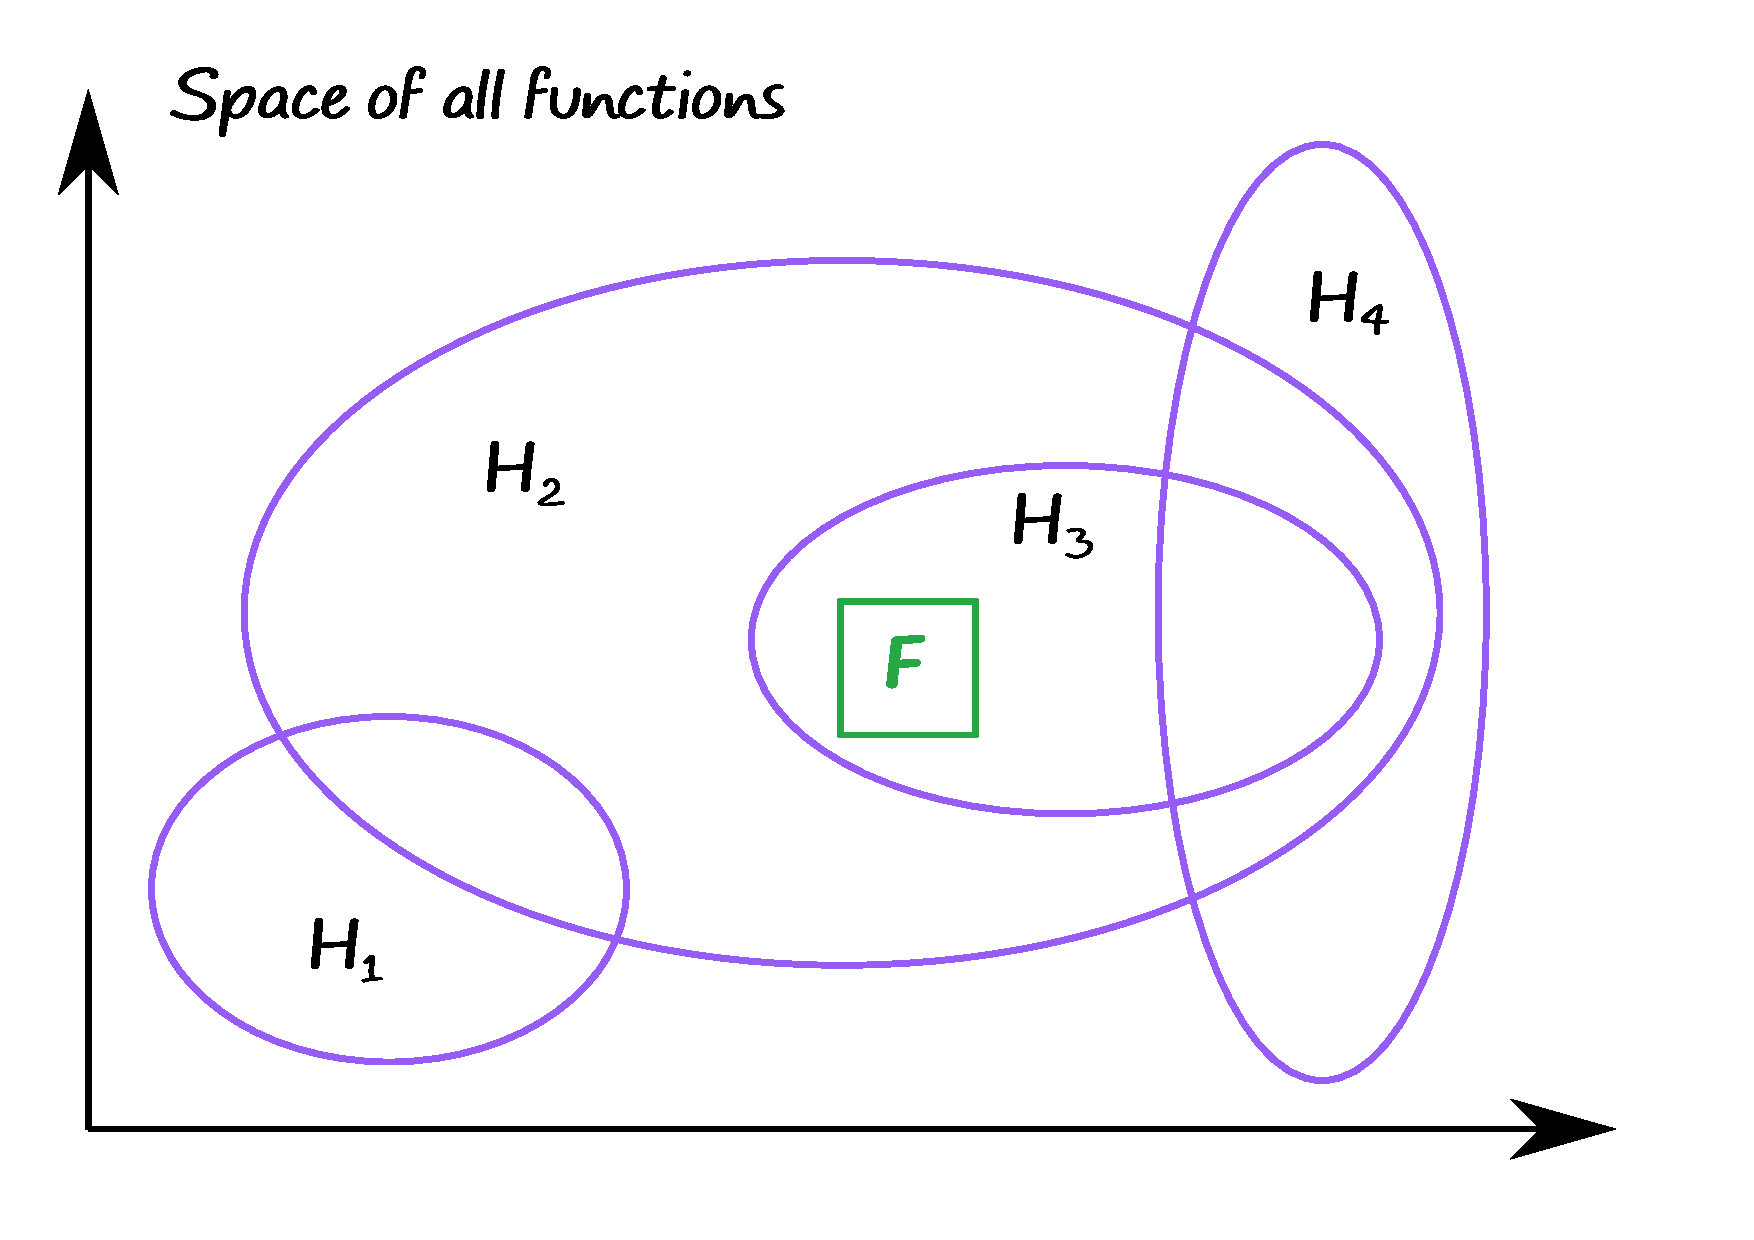
\includegraphics[width=\textwidth]{figures/space_lll.pdf} 
  \end{minipage}
\end{frame}

\begin{frame}{AIM}
  \begin{minipage}{0.45\textwidth}
    \only<1-2>{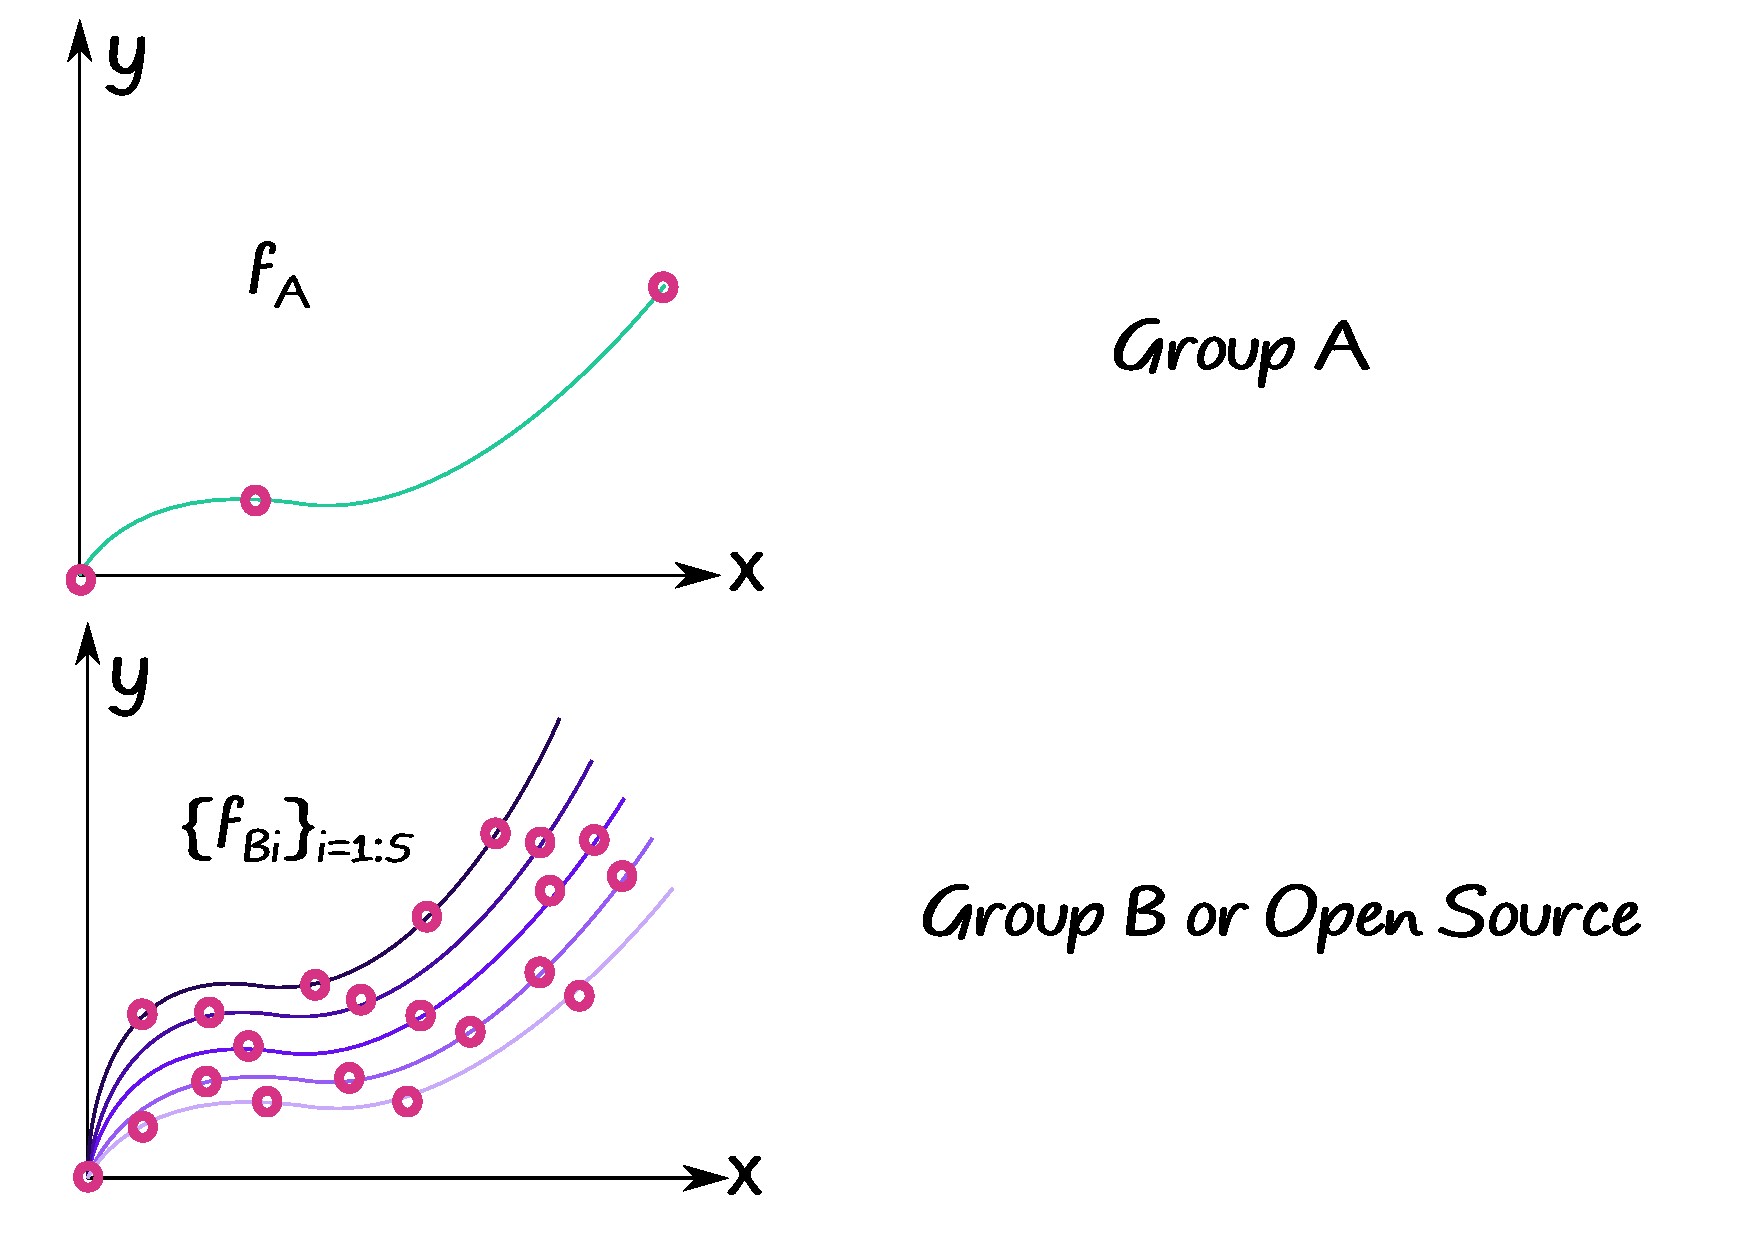
\includegraphics[width=\textwidth]{figures/meta_learning_2.pdf}}
  \end{minipage}%
  $\to$ \begin{minipage}{0.45\textwidth} \only<2>{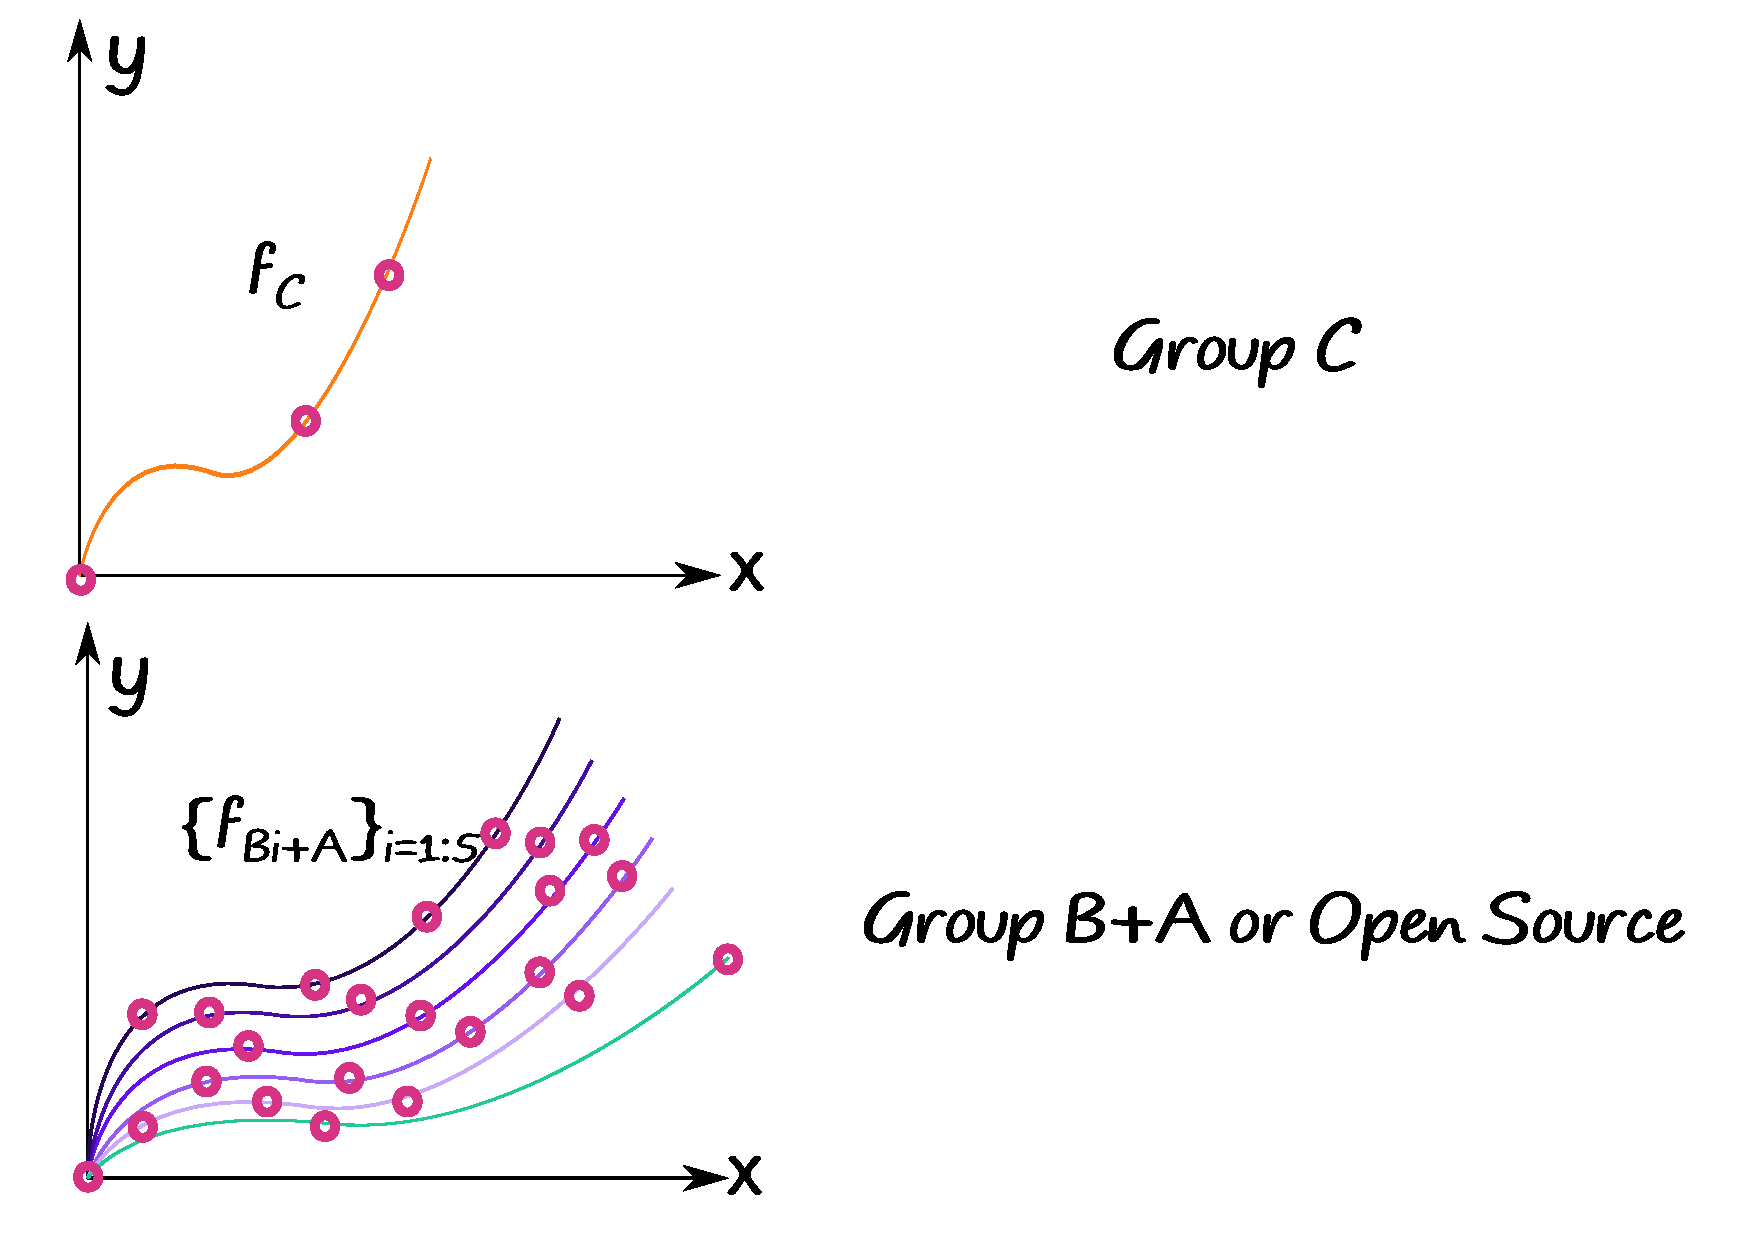
\includegraphics[width=\textwidth]{figures/meta_learning_3.pdf}}
  \end{minipage} $\dots$
\end{frame}

\begin{frame}{AIM}
  \centering
  \color{Pink} Currently:  \color{Black} Everyone (deep learning enthusiasts) obtain huge amount of data (takes ages to collect), then train their models!

  \color{Pink} Our Aim: \color{Black} Improve continuous stream of tasks  with previous tasks, and show how collaboration might decrease data and parametrization need! 
\end{frame}

\begin{frame}
	\centering
	\cont 
\end{frame}


\section{Continual Learning}
\begin{frame}{NNRelief Pruning\cite{dekhovich2022a}}
  \centering
  \begin{minipage}{\textwidth}
    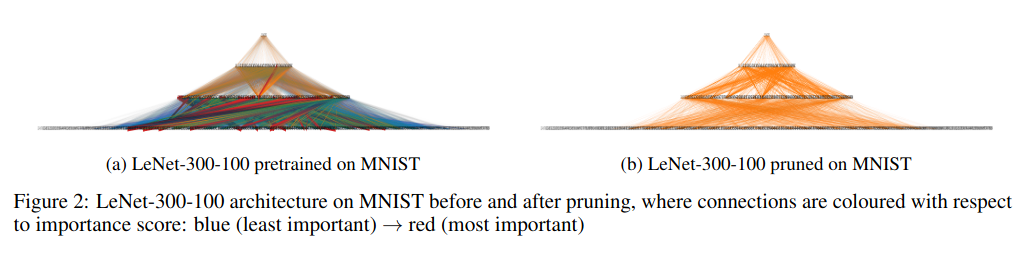
\includegraphics[width=\textwidth]{figures/nnrelief.png}
  \end{minipage}
  \begin{minipage}{\textwidth}
    \centering
    \begin{itemize}
      \item Train your NN for a task of $f:\mathcal{X}\to\mathcal{Y}$
      \item Compute the importance scores of the activations
      \item Prune them with a pre-defined tolerance
    \end{itemize}
  \end{minipage}
\end{frame}

\begin{frame}{Continual Prune \& Select\cite{dekhovich2022}}
  \begin{minipage}{0.5\textwidth}
    \begin{itemize}
      \item Given a task $f_i:|\mathcal{X}\to\mathcal{Y}$ find sub-network $\mathcal{N}_i$ inside a given NN $\bigcup_{i=1}^M \mathcal{N}_i $
      \item Prune with NNRelief
      \item Fix the sub-network parameters and repeat the same procedure for $f_{i+1}$
      \item In the end you end up with task specific networks 
    \end{itemize}
  \end{minipage}%
  \begin{minipage}{0.5\textwidth}
    \centering
    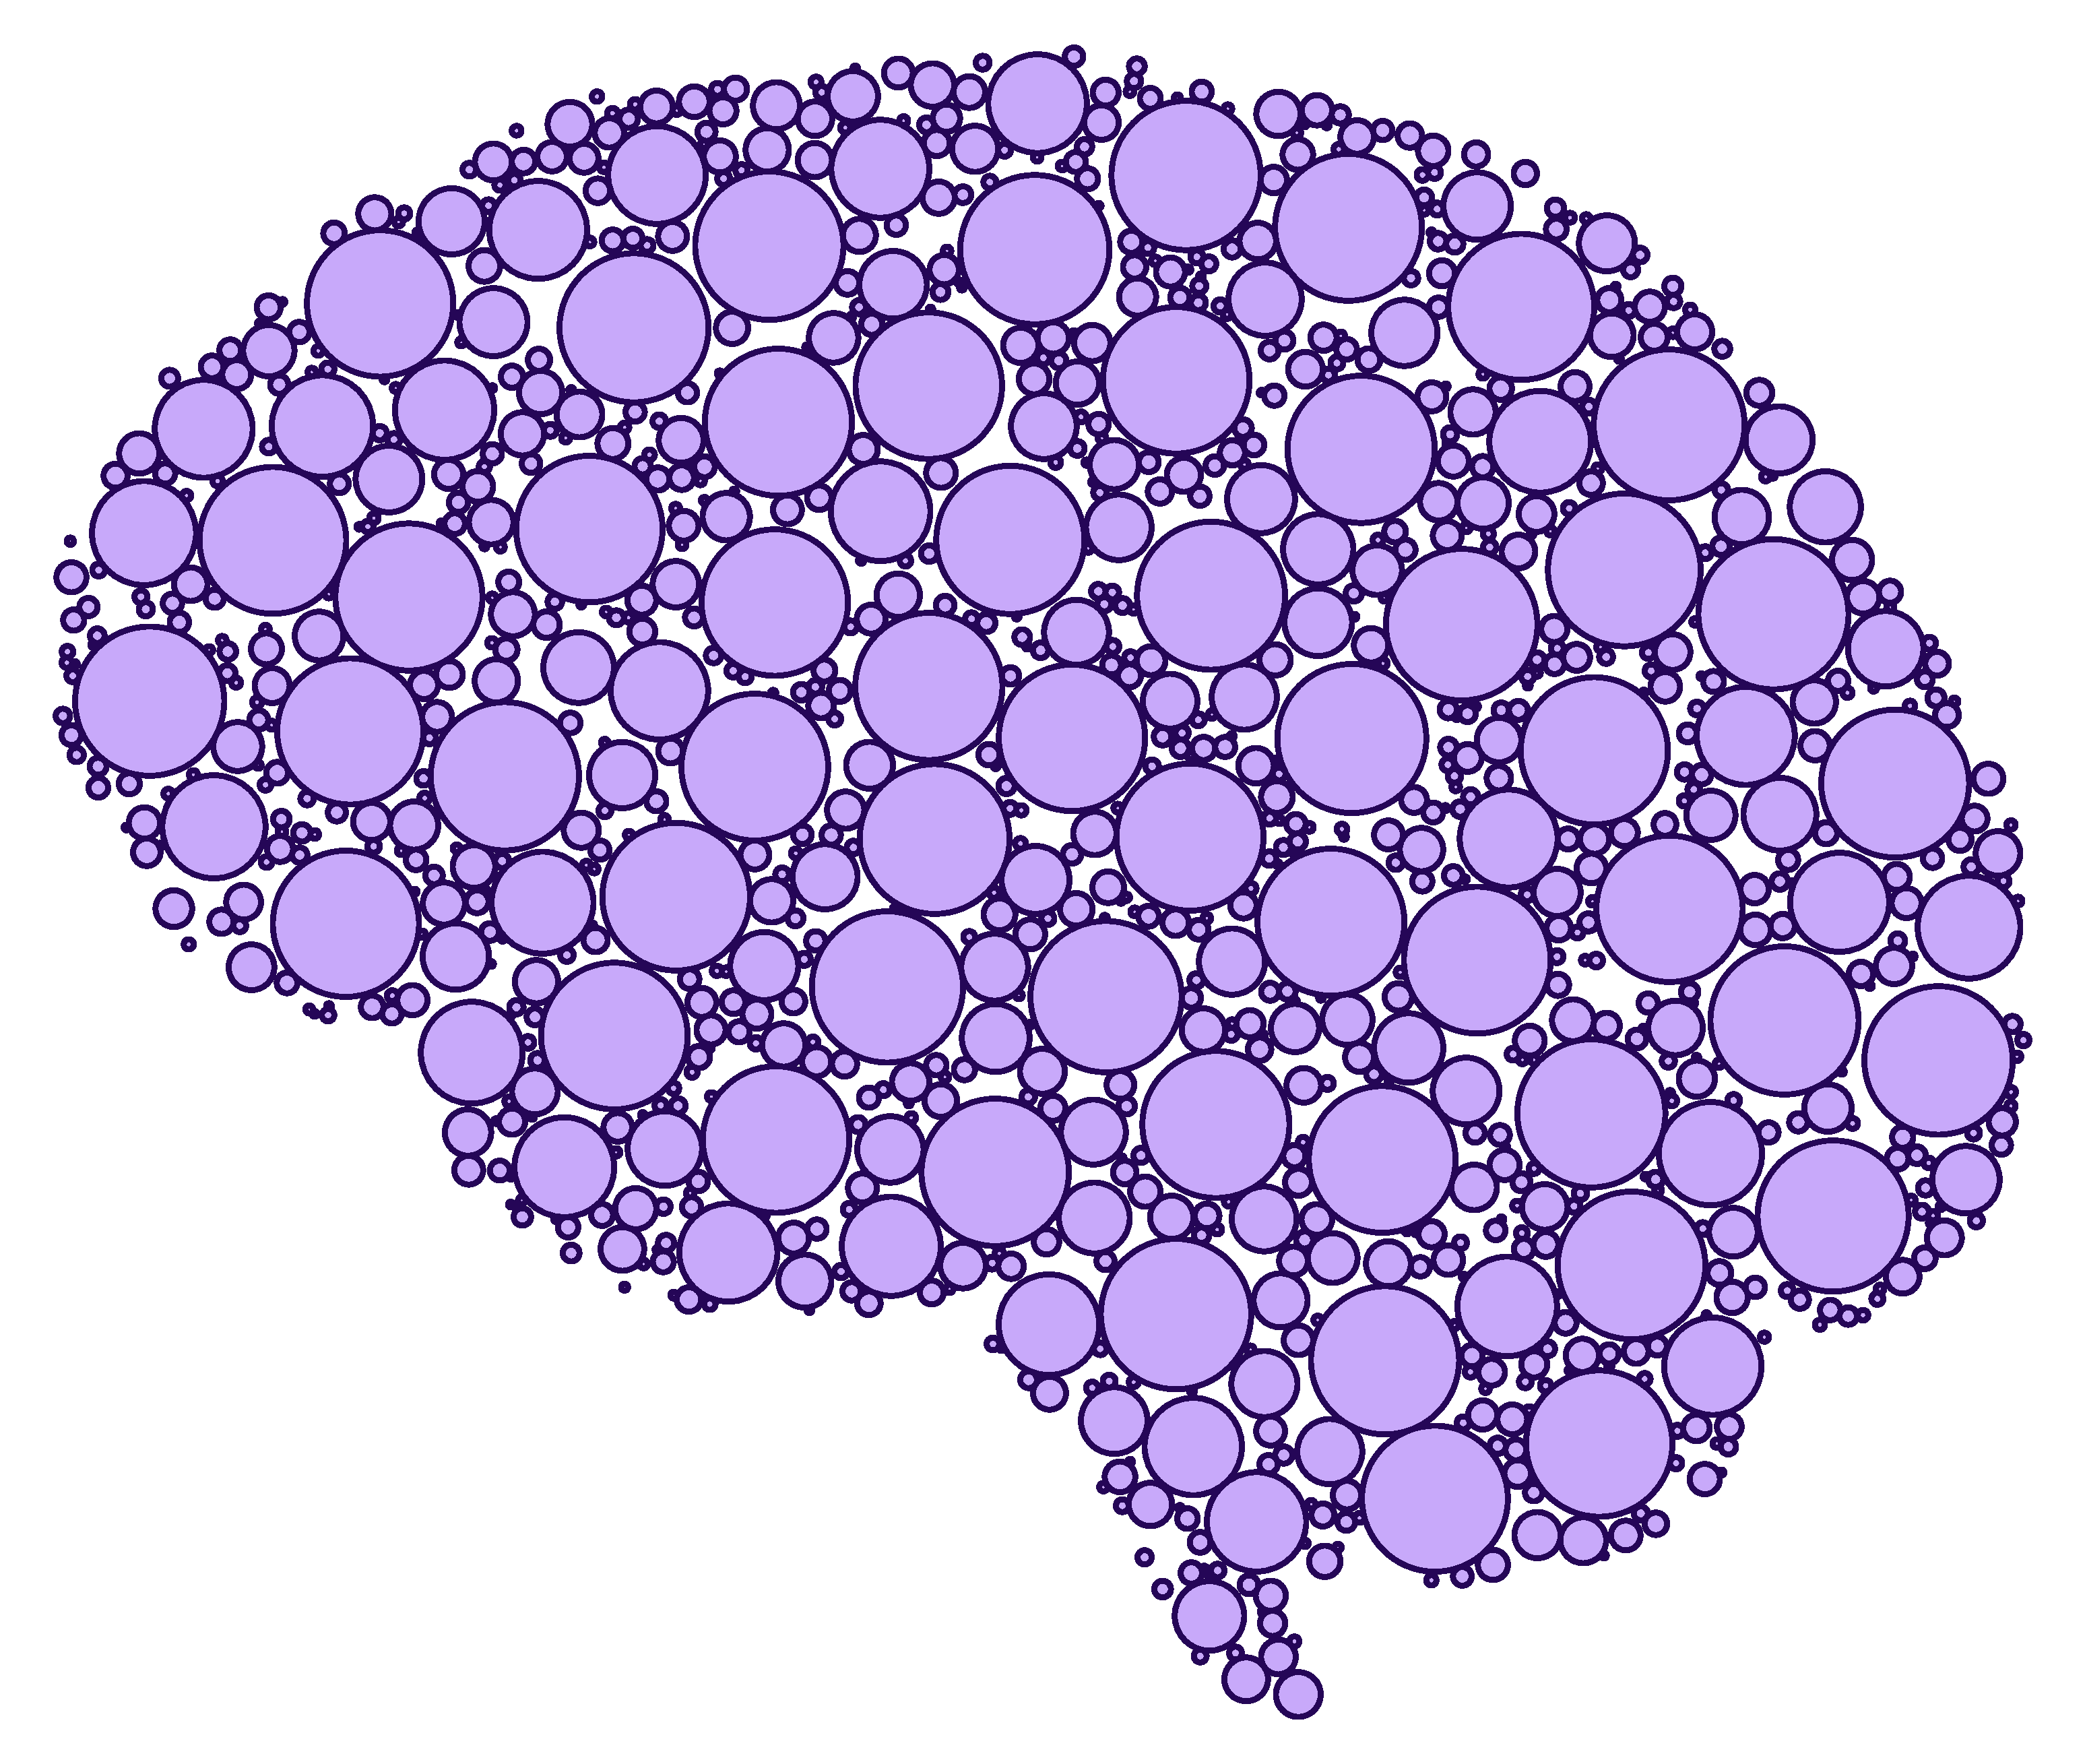
\includegraphics[width=0.9\textwidth]{figures/brain.pdf}
  \end{minipage}
\end{frame}

\begin{frame}
	\centering
	\app
\end{frame}

\section{Application}
\begin{frame}{Plasticity}
  \begin{minipage}{0.5\textwidth}
    \only<1>
    {
      Plastic Constitutive Law:
      \begin{itemize}
        \item Path dependent problem
        \item $\boldsymbol{\sigma}=\mathcal{C}(\epsilon, t, \boldsymbol{\theta})$
        \item $\sigma\in\mathbb{R}^3$ and $\epsilon\in\mathbb{R}^3$
      \end{itemize}
    }
    \only<2>
    {
      As a continual learning problem:
      \begin{itemize}
        \item $\boldsymbol{\theta}$ Determines the different tasks
        \item Try to learn $\mathcal{C}$
        \item Given $\{\boldsymbol{\sigma}^{\boldsymbol{\theta_i}}_{t=1:T},\boldsymbol{\epsilon}^{\boldsymbol{\theta_i}}_{t=1:T}\}_i=1,M$
      \end{itemize}
    }
  \end{minipage}%
  \begin{minipage}{0.5\textwidth}
    \centering
    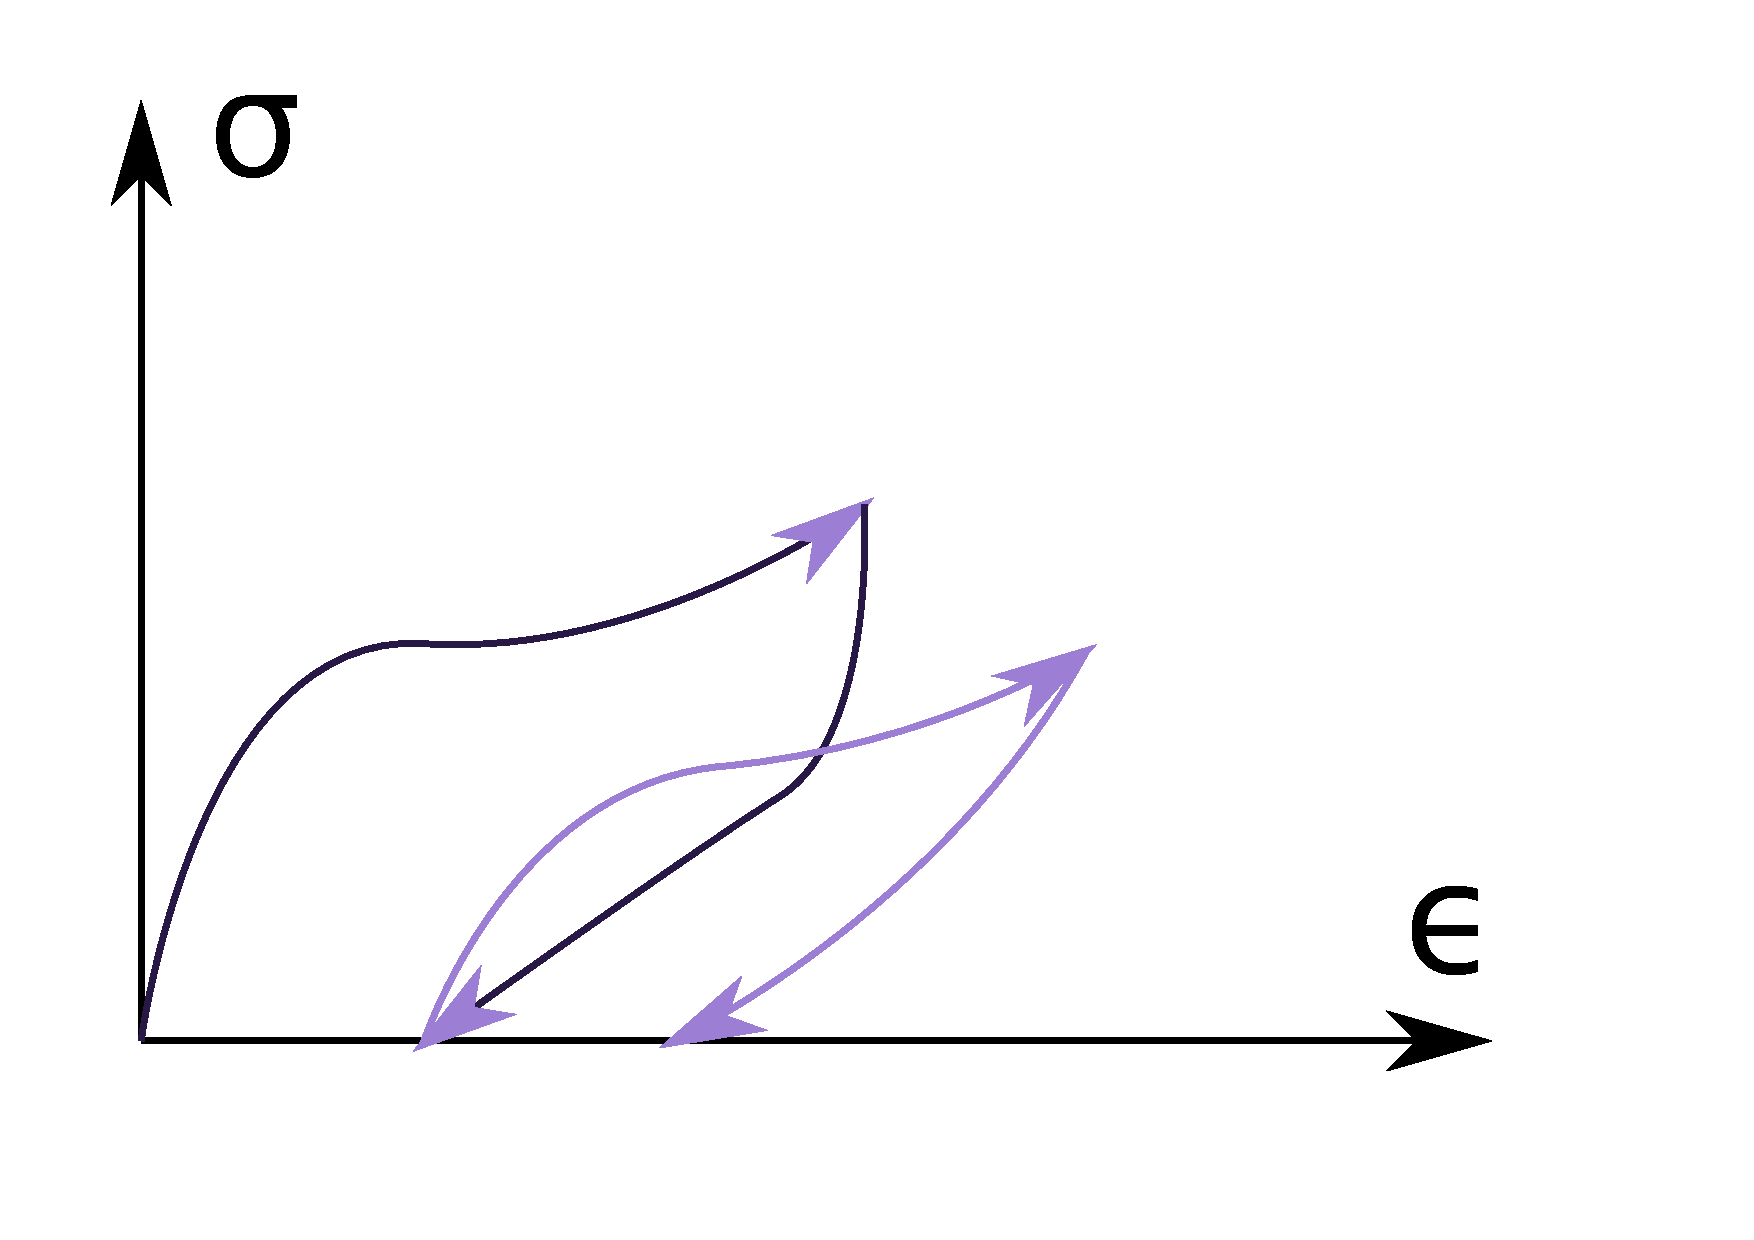
\includegraphics[width=0.9\textwidth]{figures/plastic.pdf}
  \end{minipage}
\end{frame}

\begin{frame}{Problem}
    \begin{itemize}
      \item 4 Tasks with 800 available train paths and 200 test paths (sampled from Gaussian Process) 
      \item Assume the task-ID is known
    \end{itemize}
  \begin{minipage}{0.5\textwidth}
    \centering
    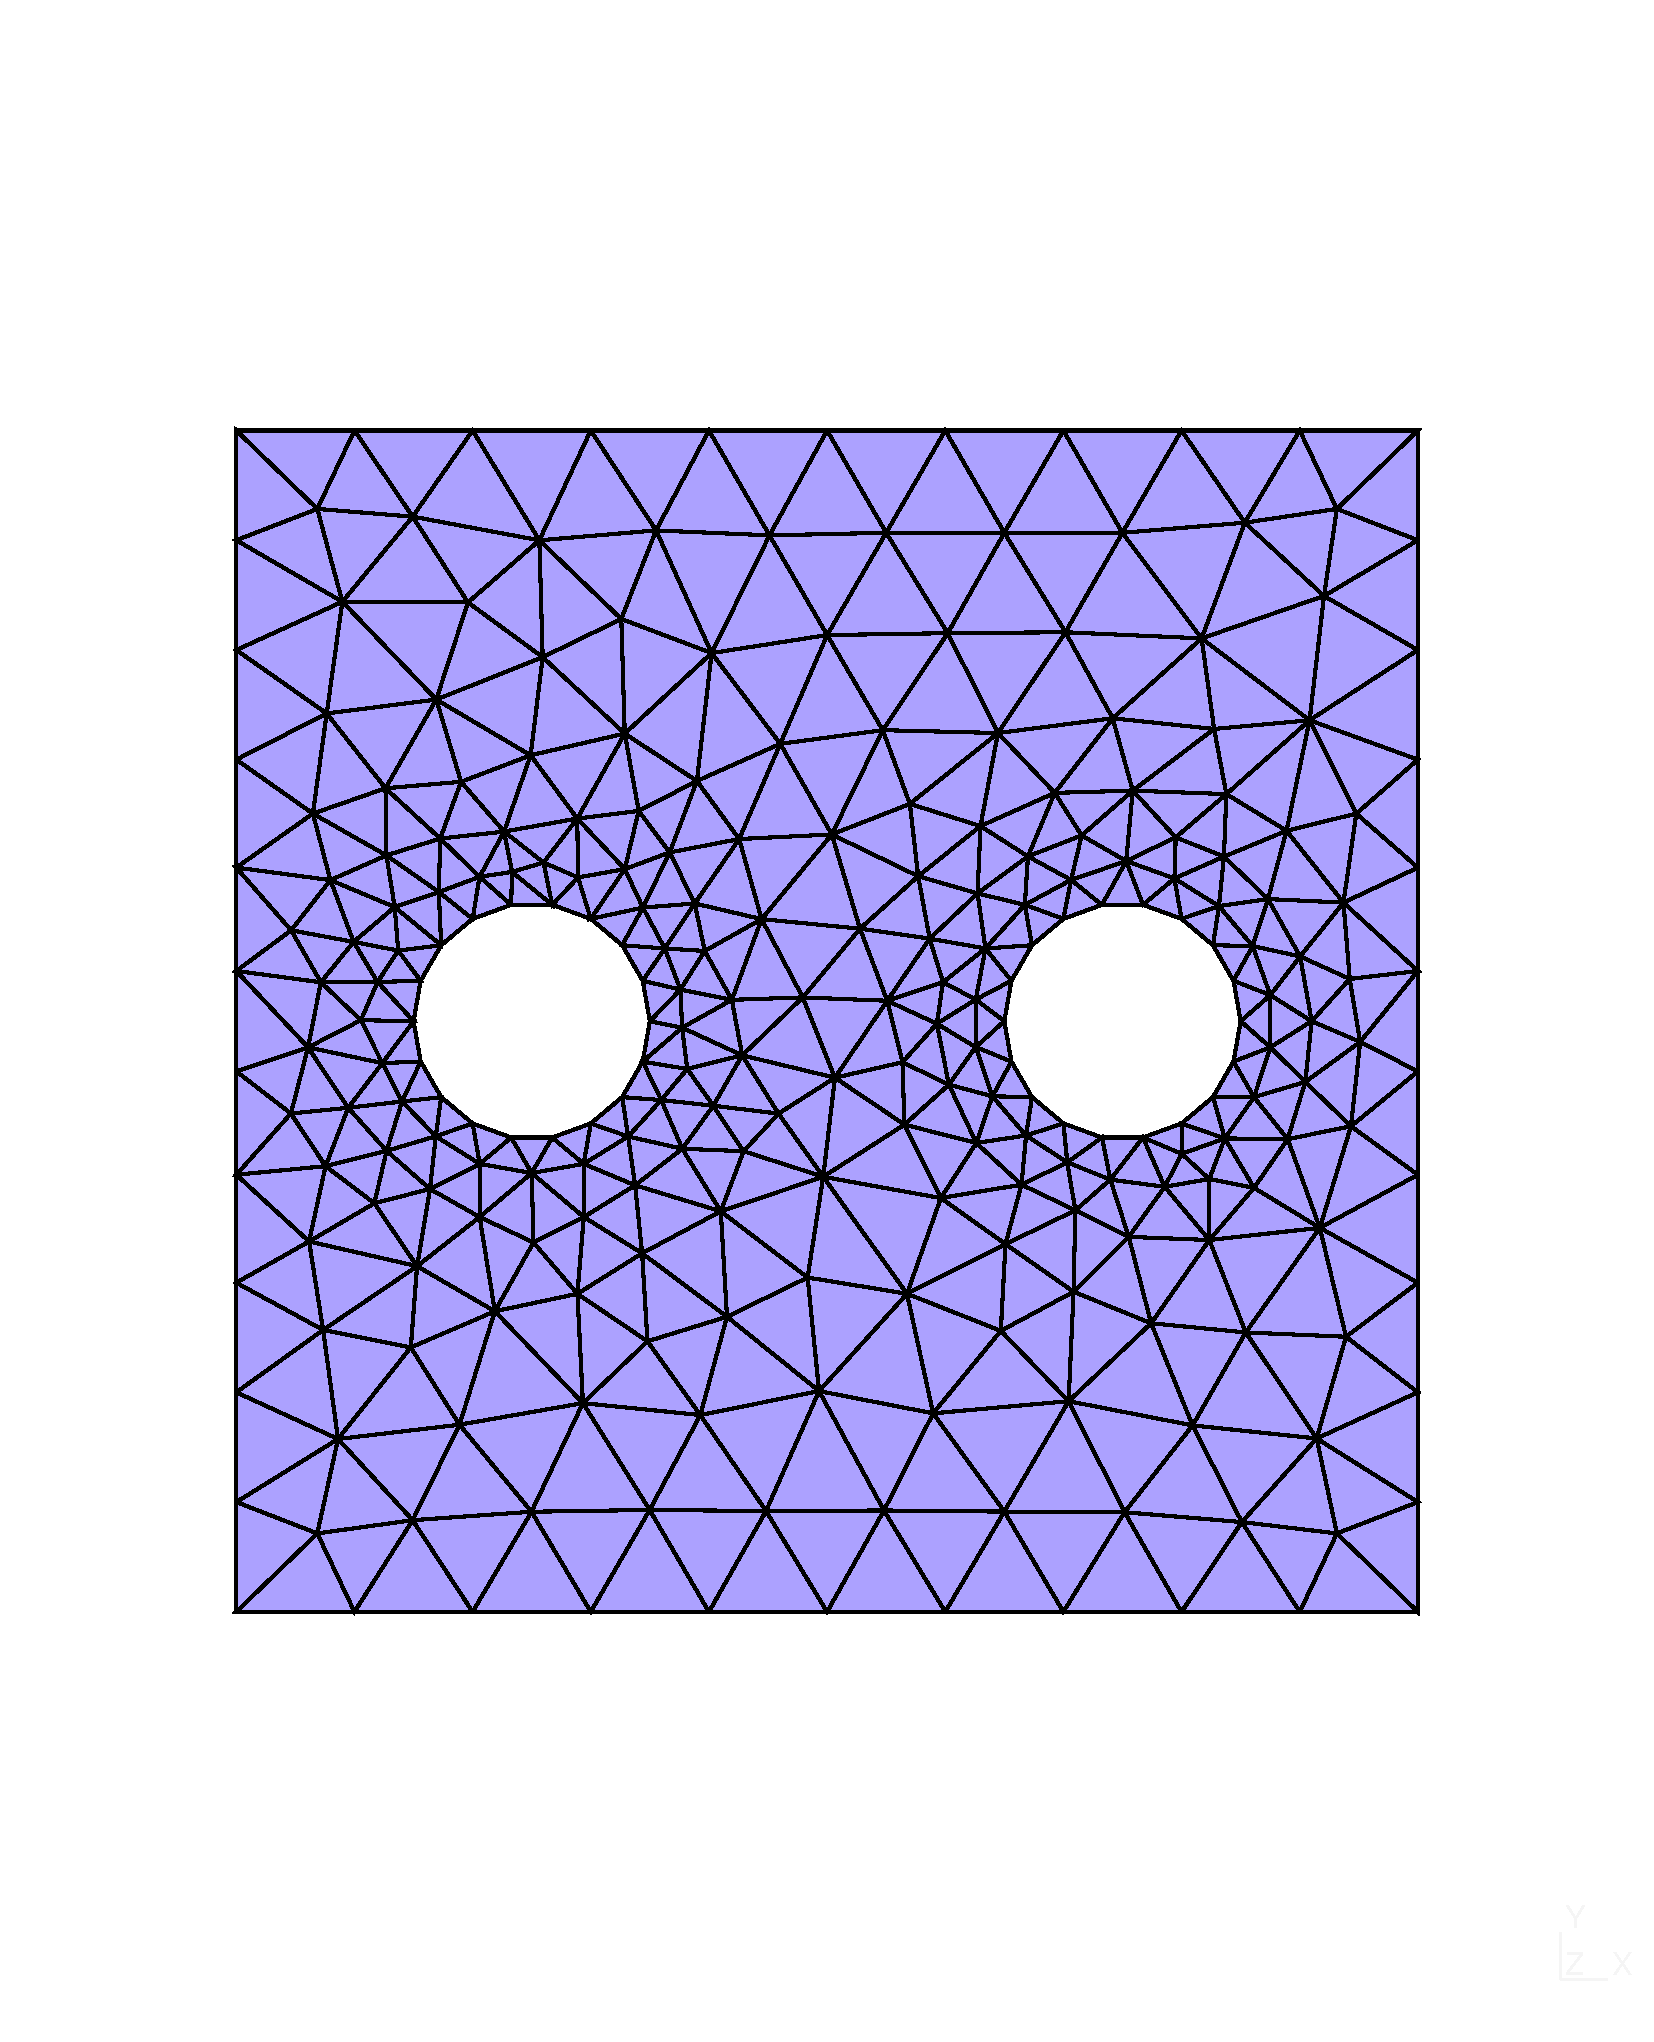
\includegraphics[width=0.3\textwidth]{figures/2_on_x.pdf}%
    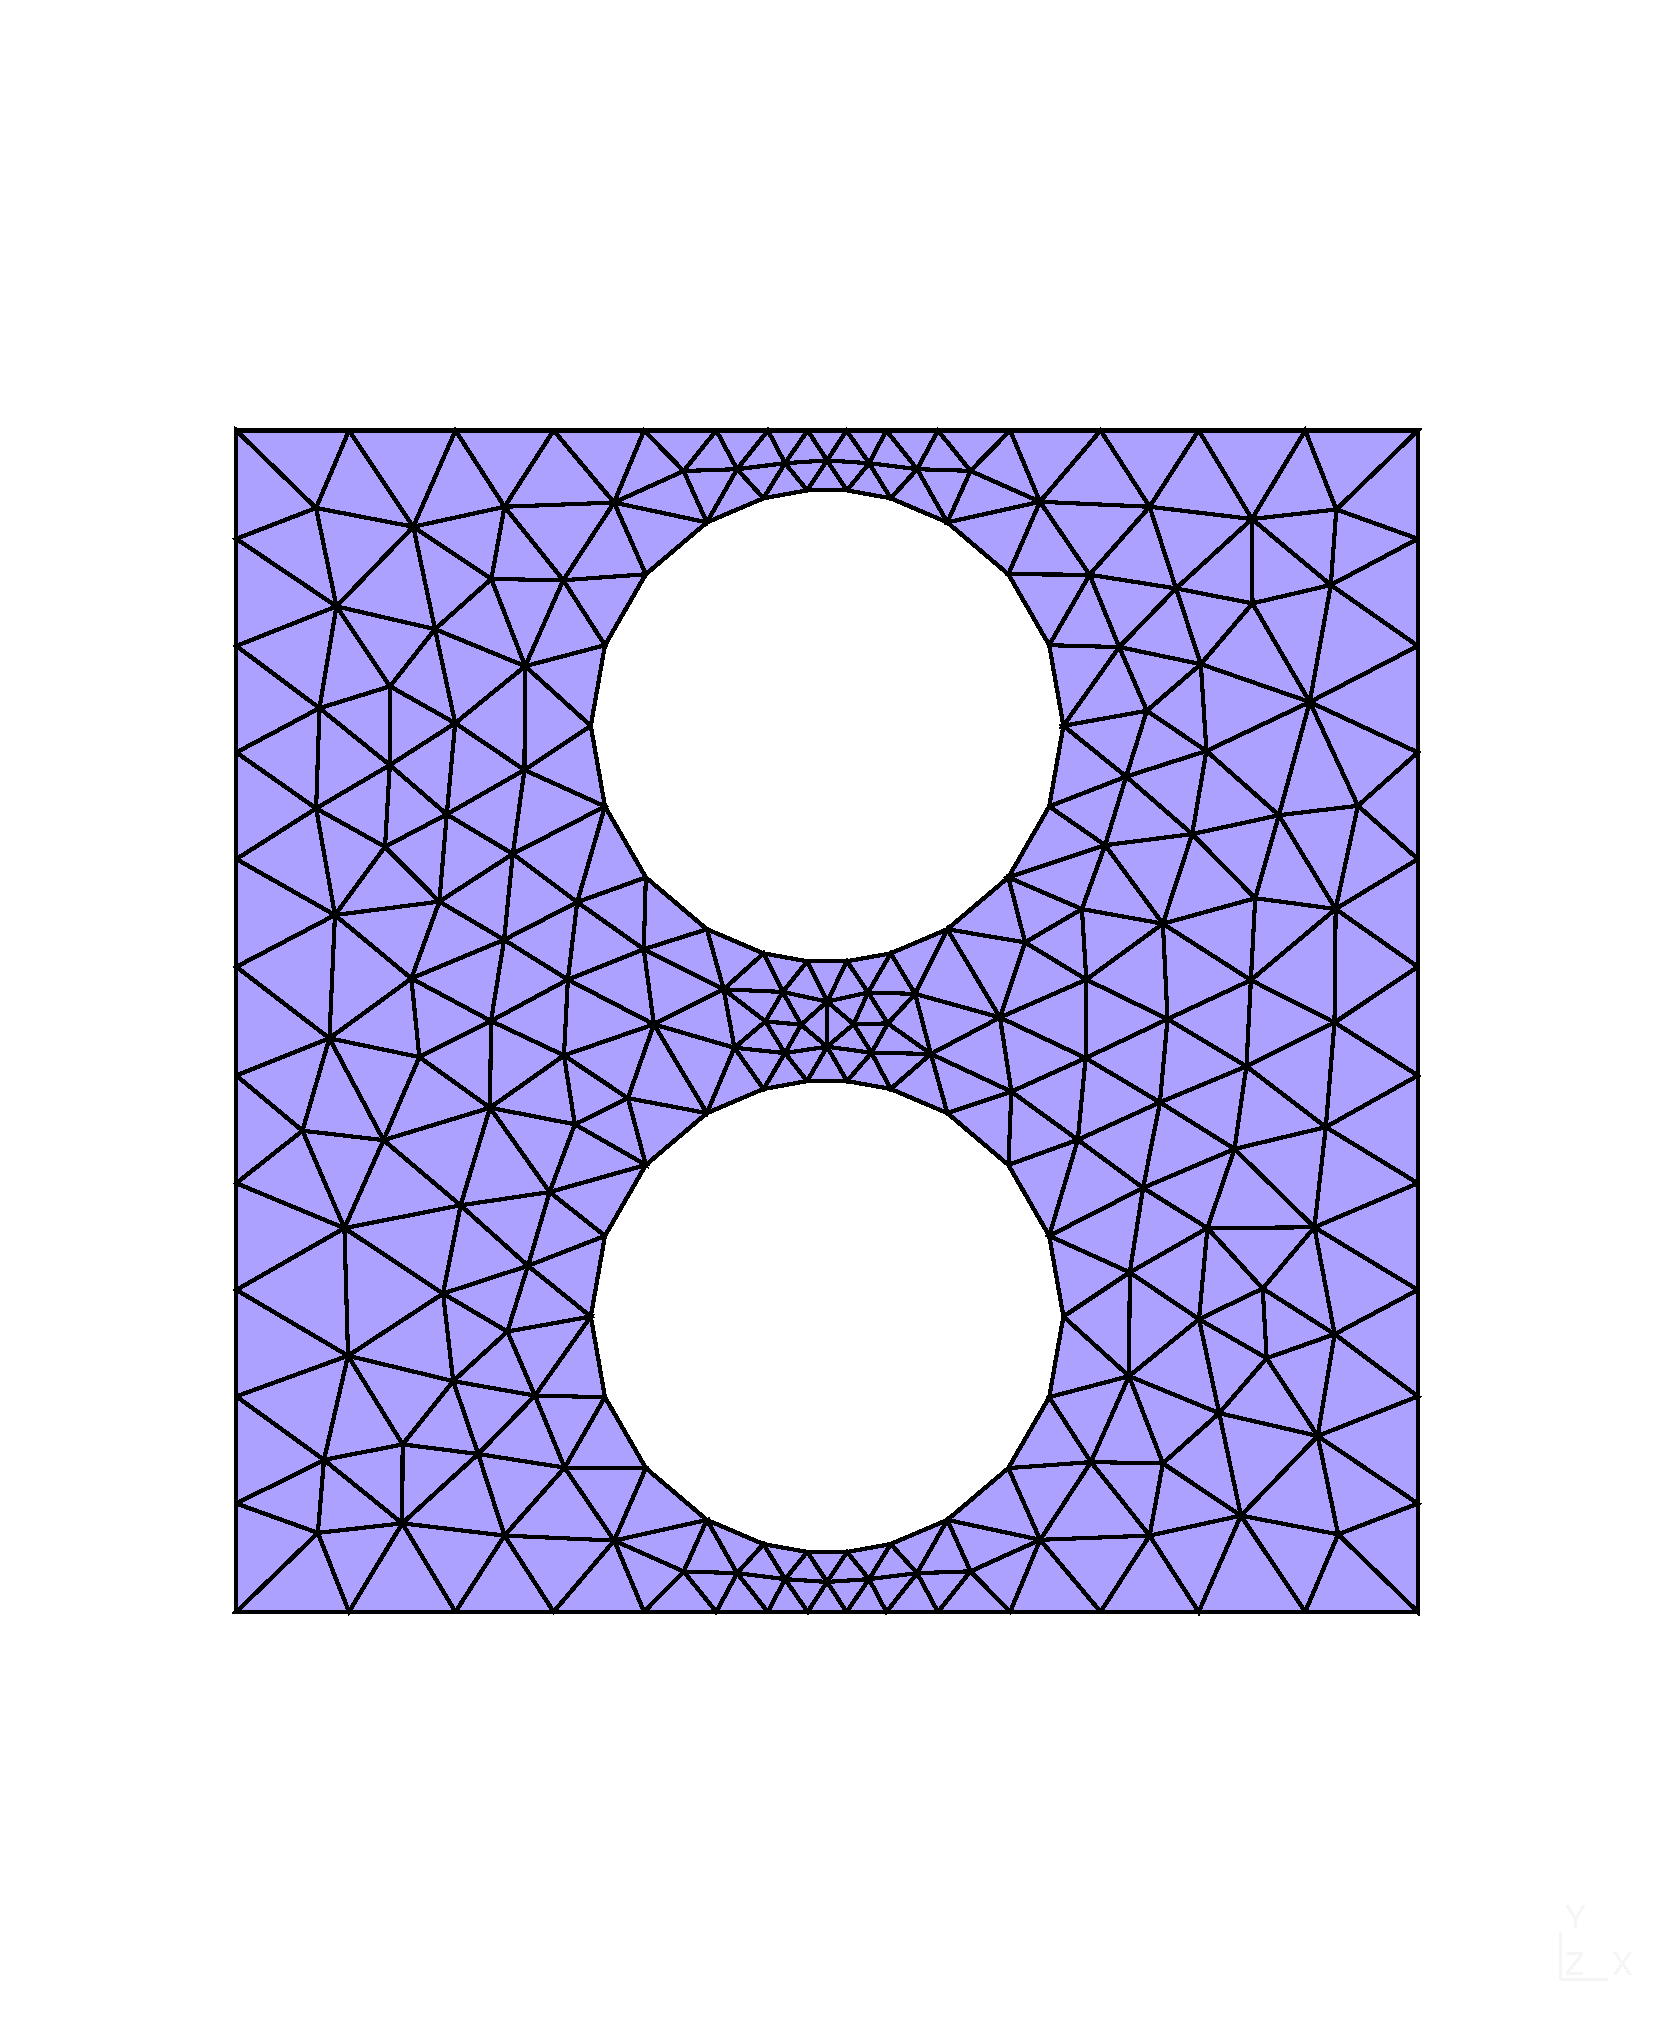
\includegraphics[width=0.3\textwidth]{figures/2_on_y.pdf}
    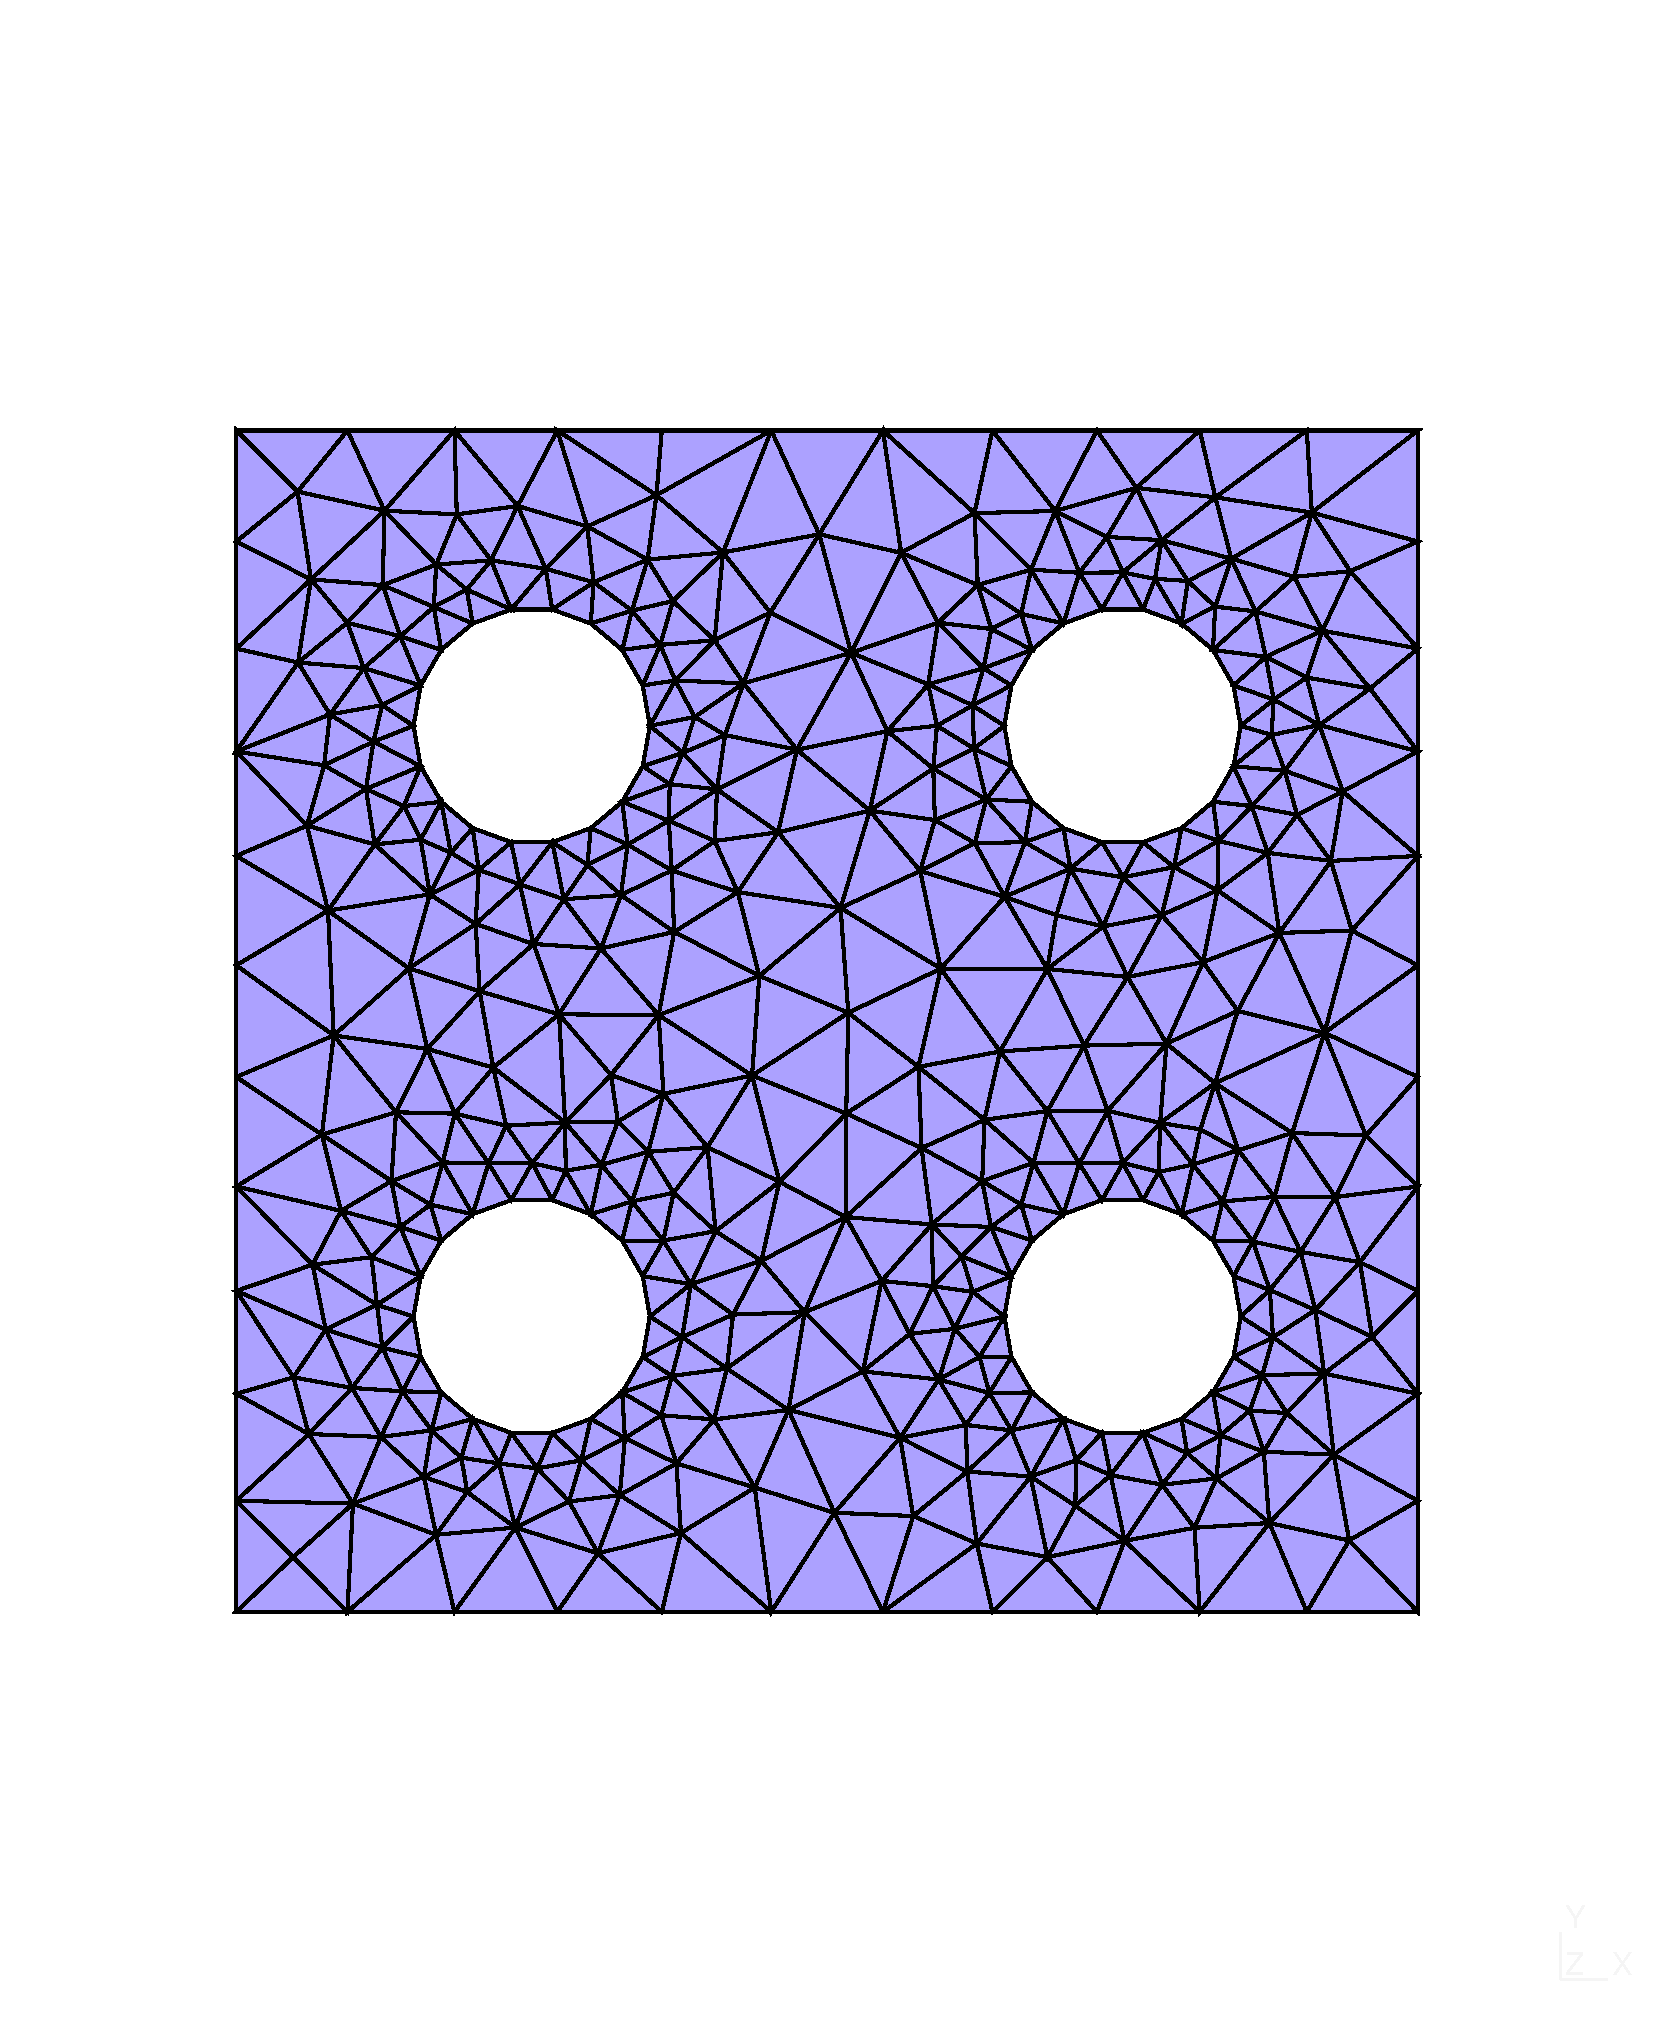
\includegraphics[width=0.3\textwidth]{figures/4_diagonal.pdf}%
    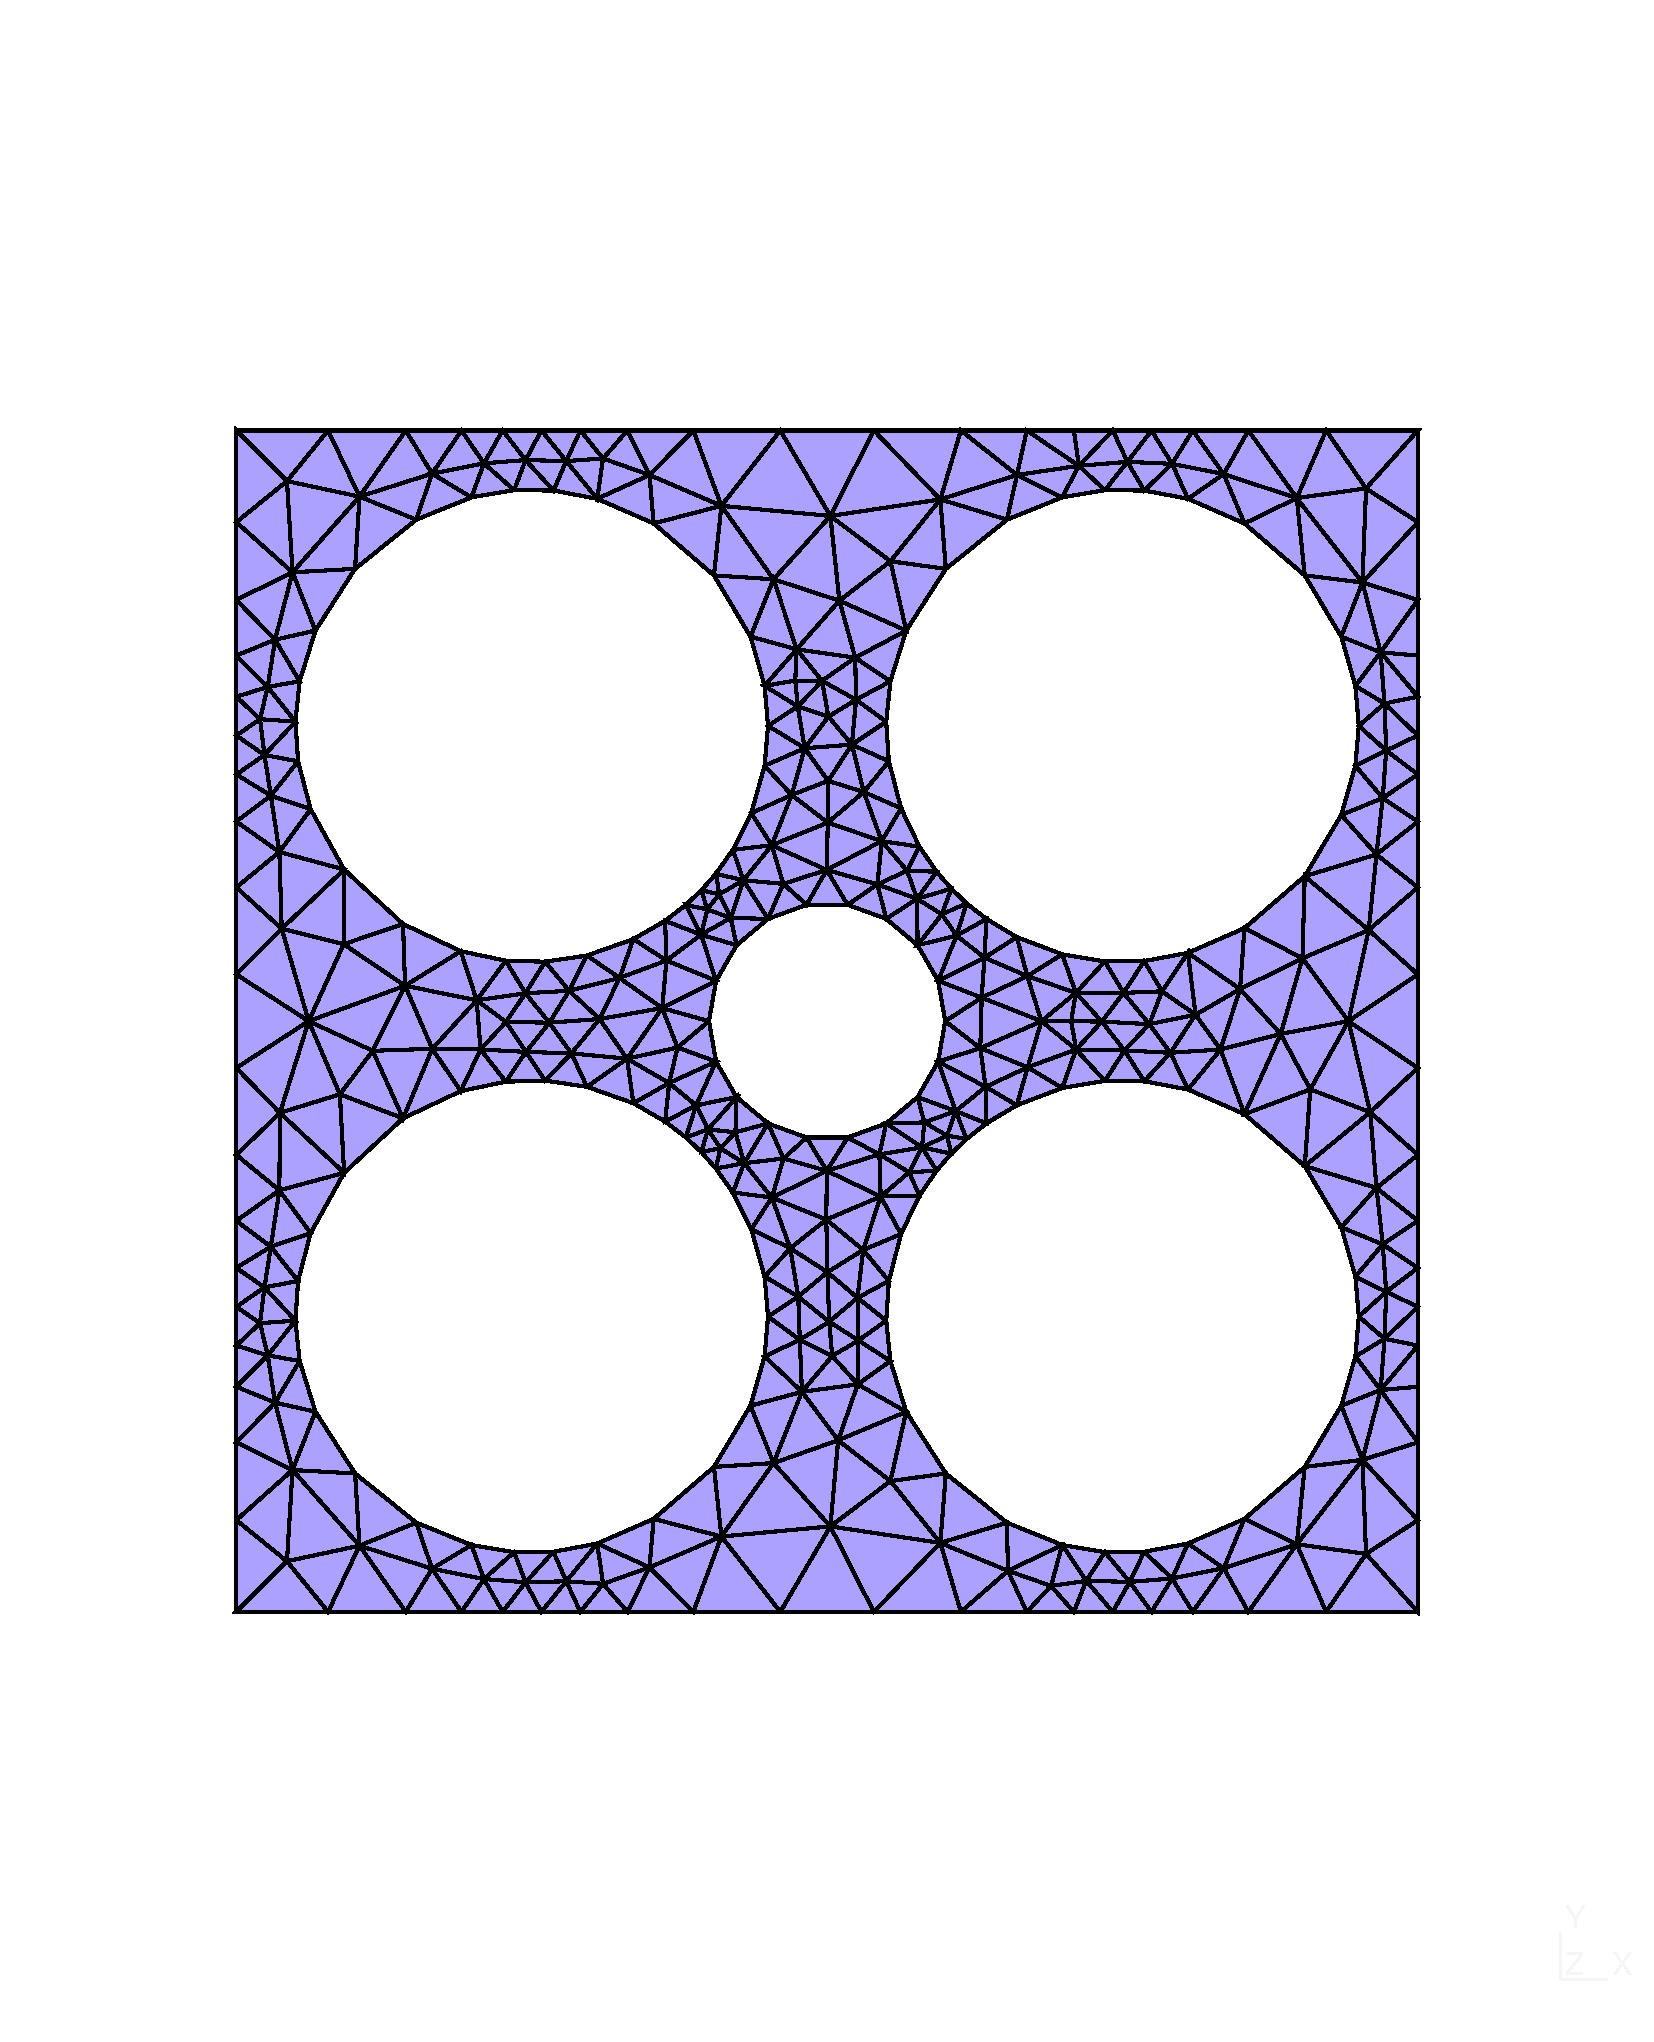
\includegraphics[width=0.3\textwidth]{figures/5_star.pdf}
  \end{minipage}%
  \begin{minipage}{0.5\textwidth}
    \centering
    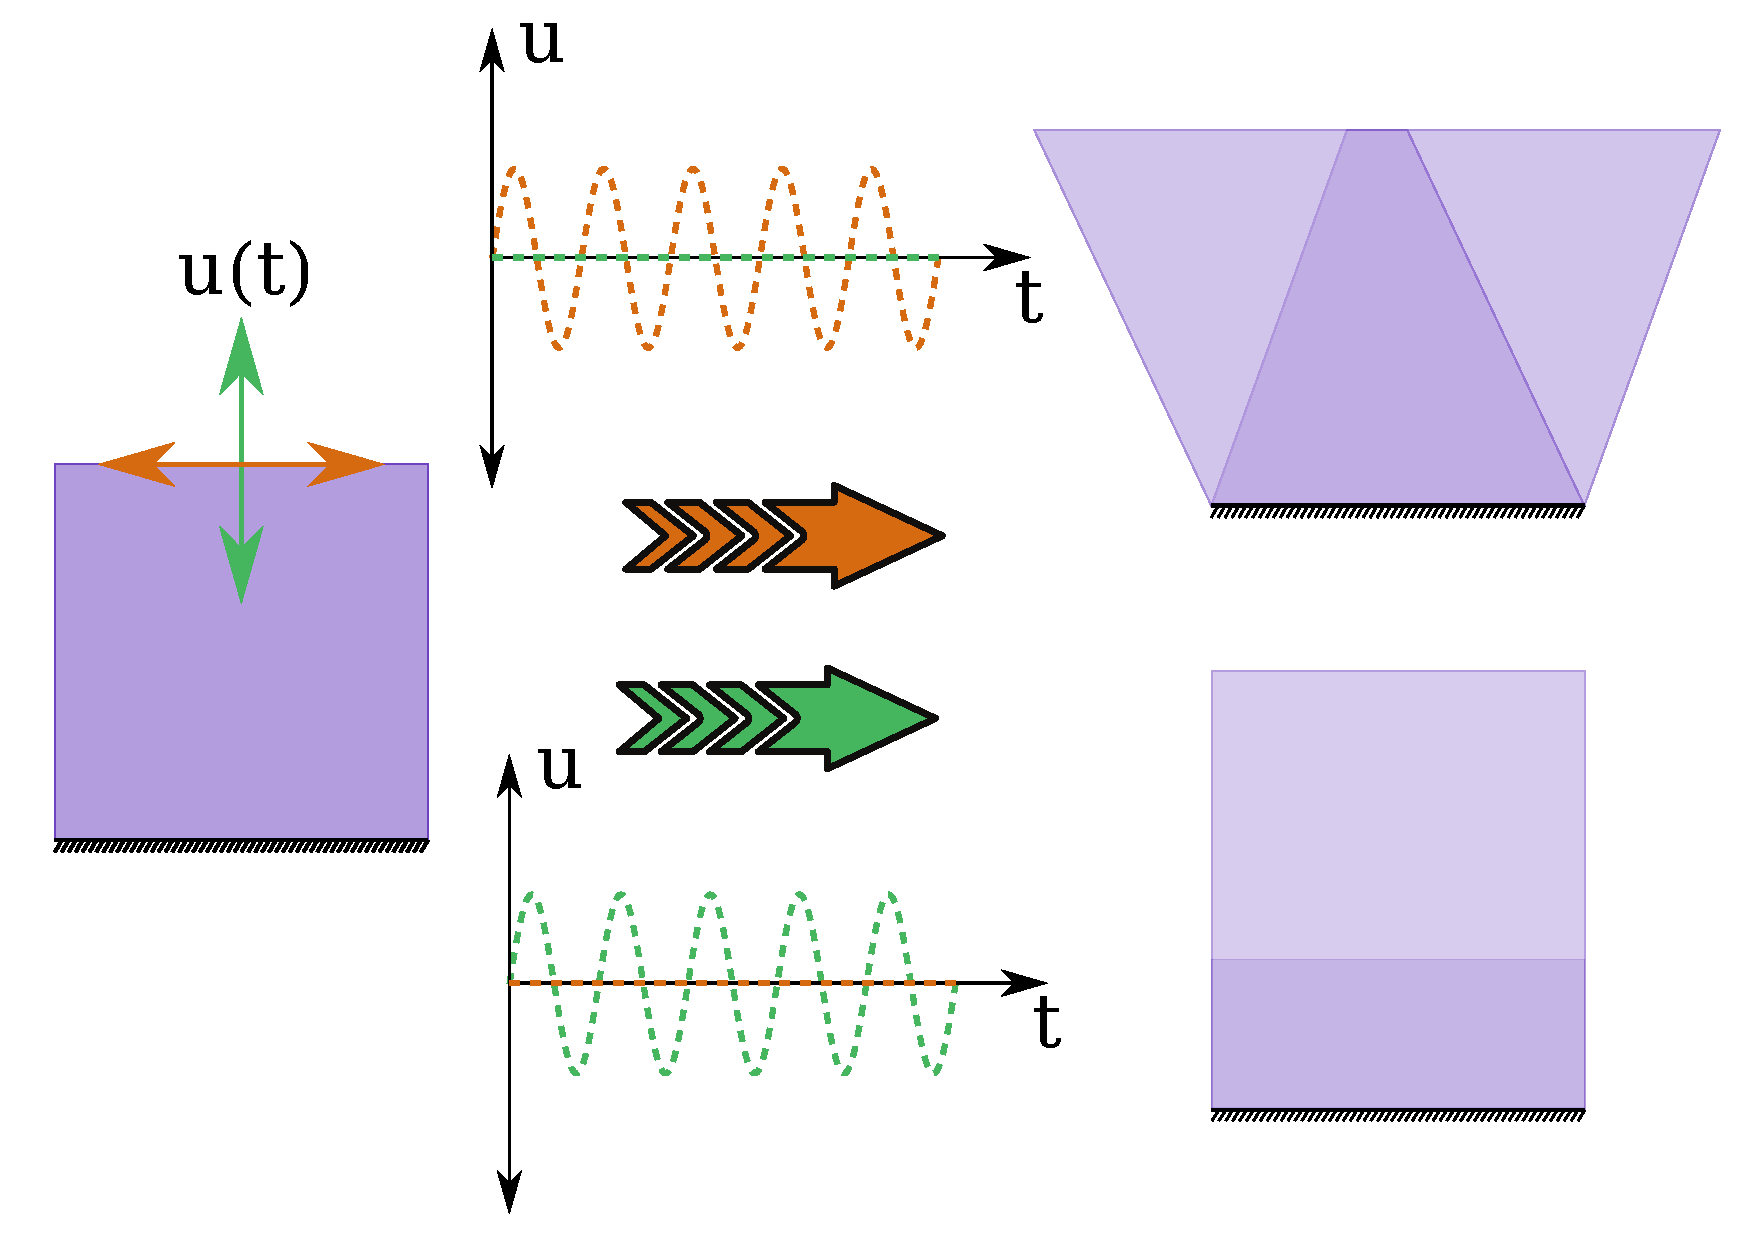
\includegraphics[width=0.9\textwidth]{figures/problem.pdf}
  \end{minipage}
\end{frame}

\begin{frame}{Difference of Tasks}
    \begin{itemize}
      \item Same strain paths for each task
      \item Different strain localization 
    \end{itemize}
    \centering
    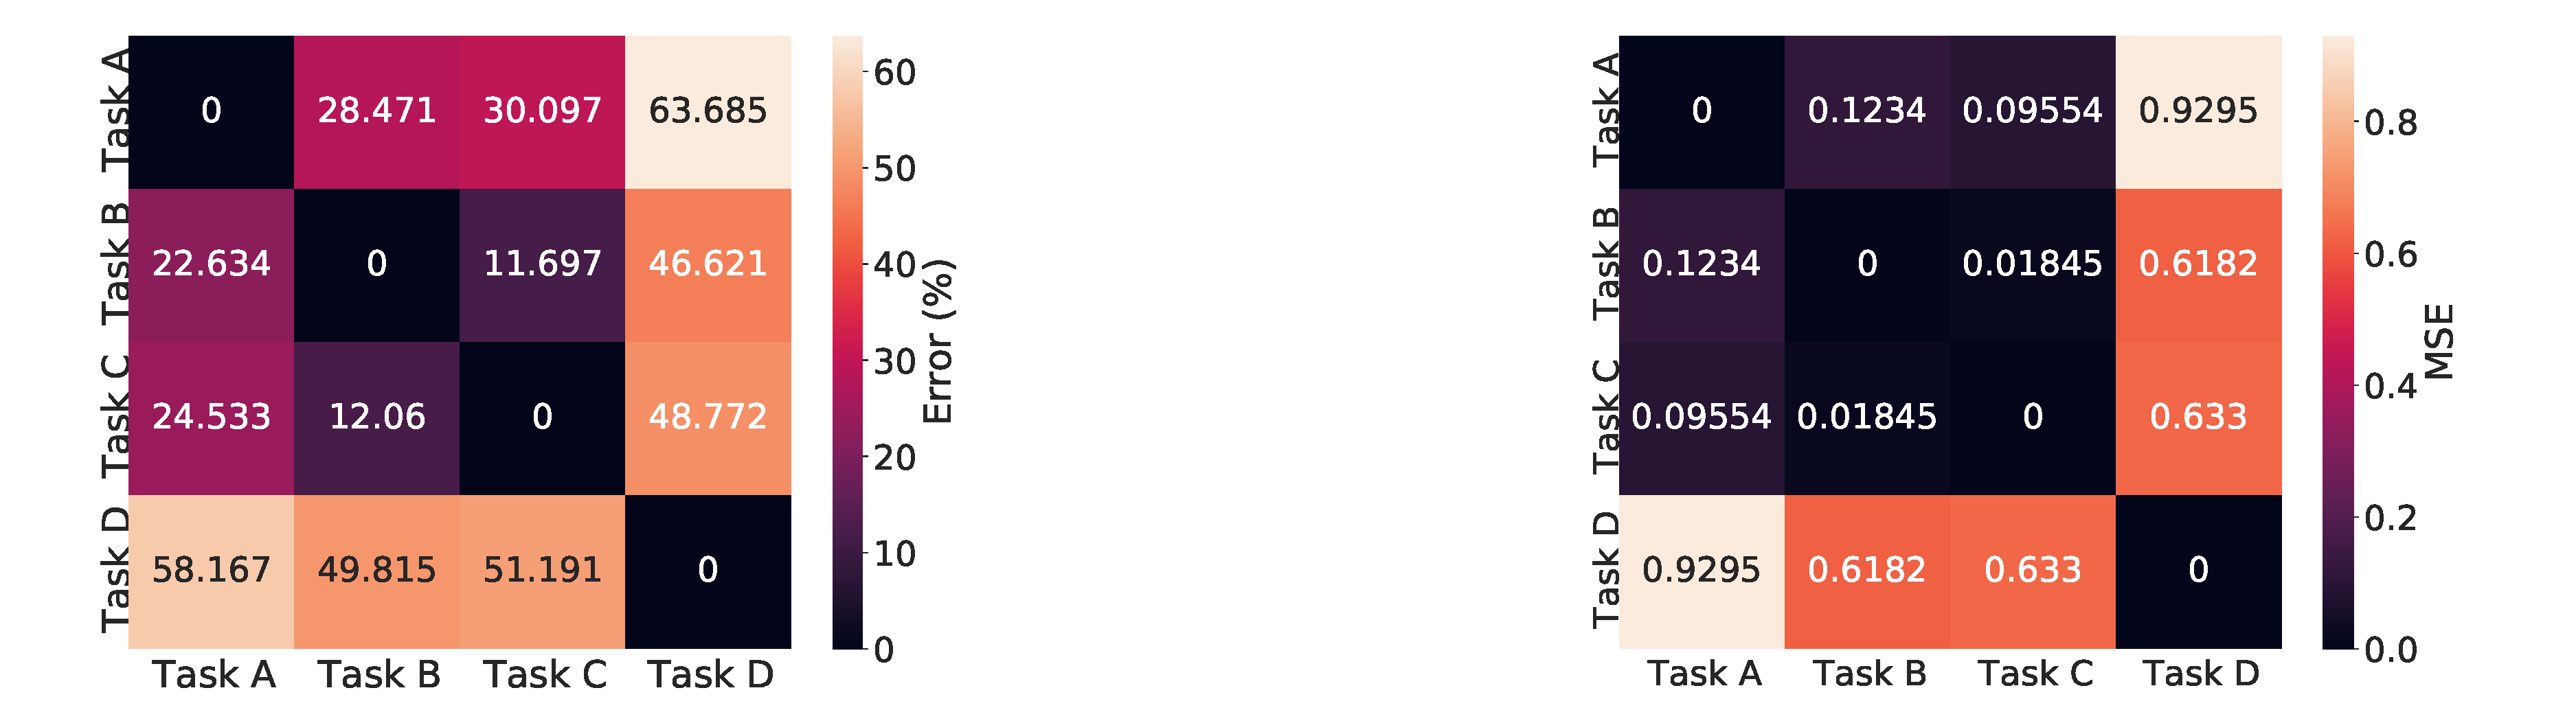
\includegraphics[width=0.9\textwidth]{figures/diff.pdf}
\end{frame}

\begin{frame}{Some Hyper-parameters}
    \begin{itemize}
      \item Not the best...
      \item 2 cells GRU with 128 hidden size
    \end{itemize}
  \centering
  \begin{tabular}{|c|c|c|c|c|c|}
    \hline
   epochs & lr & wd & pruning iter & pruning param $\alpha$ & retrain epochs  \\ % Table header row
  \hline
    1000 & 0.01 & $10^{-6}$ & 1 & 0.95 & 200 \\
  \hline
  \end{tabular}
\end{frame}

\begin{frame}{Example}
    \begin{itemize}
      \item With 800 training paths for all tasks
    \end{itemize}
    \centering
    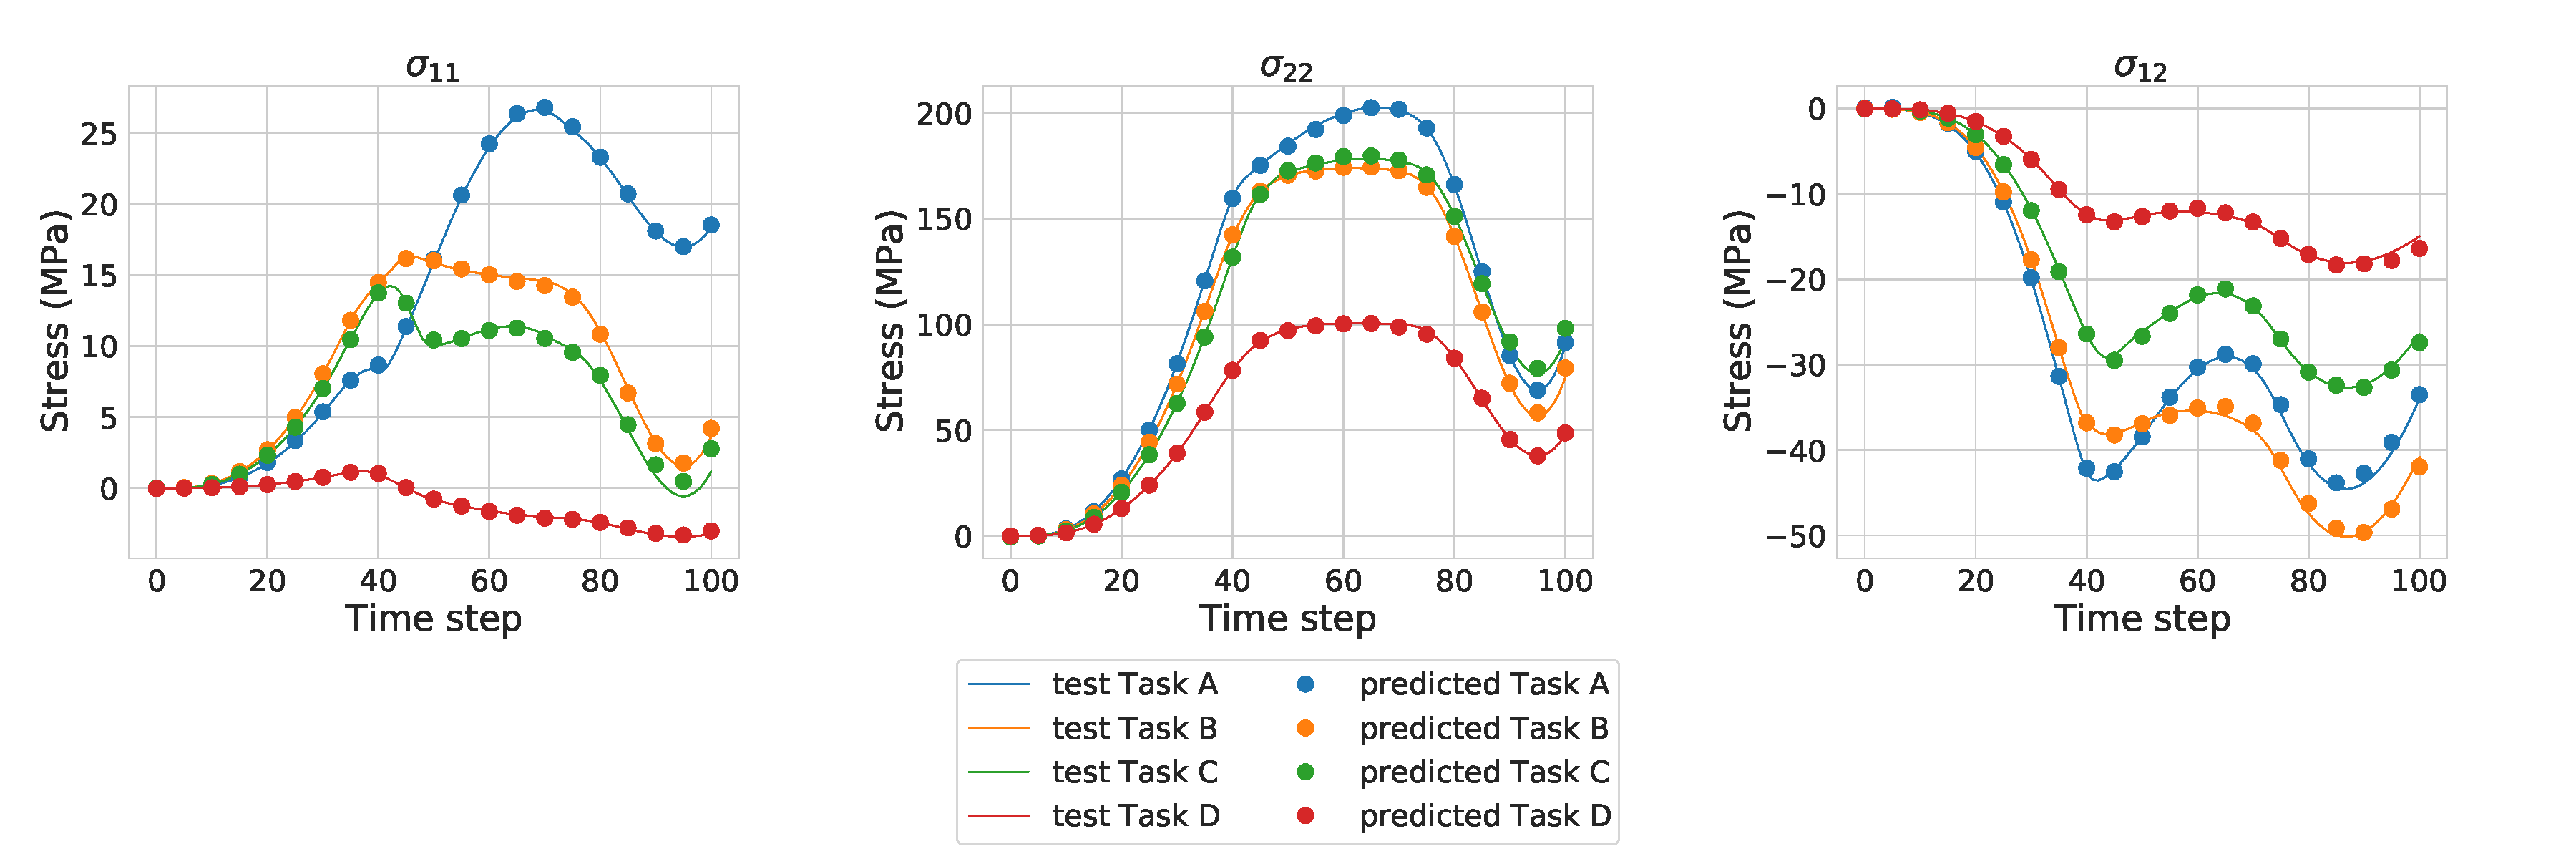
\includegraphics[width=\textwidth]{figures/example_paths.pdf}
\end{frame}

\begin{frame}{Compare with Standard Learning}
    \centering
    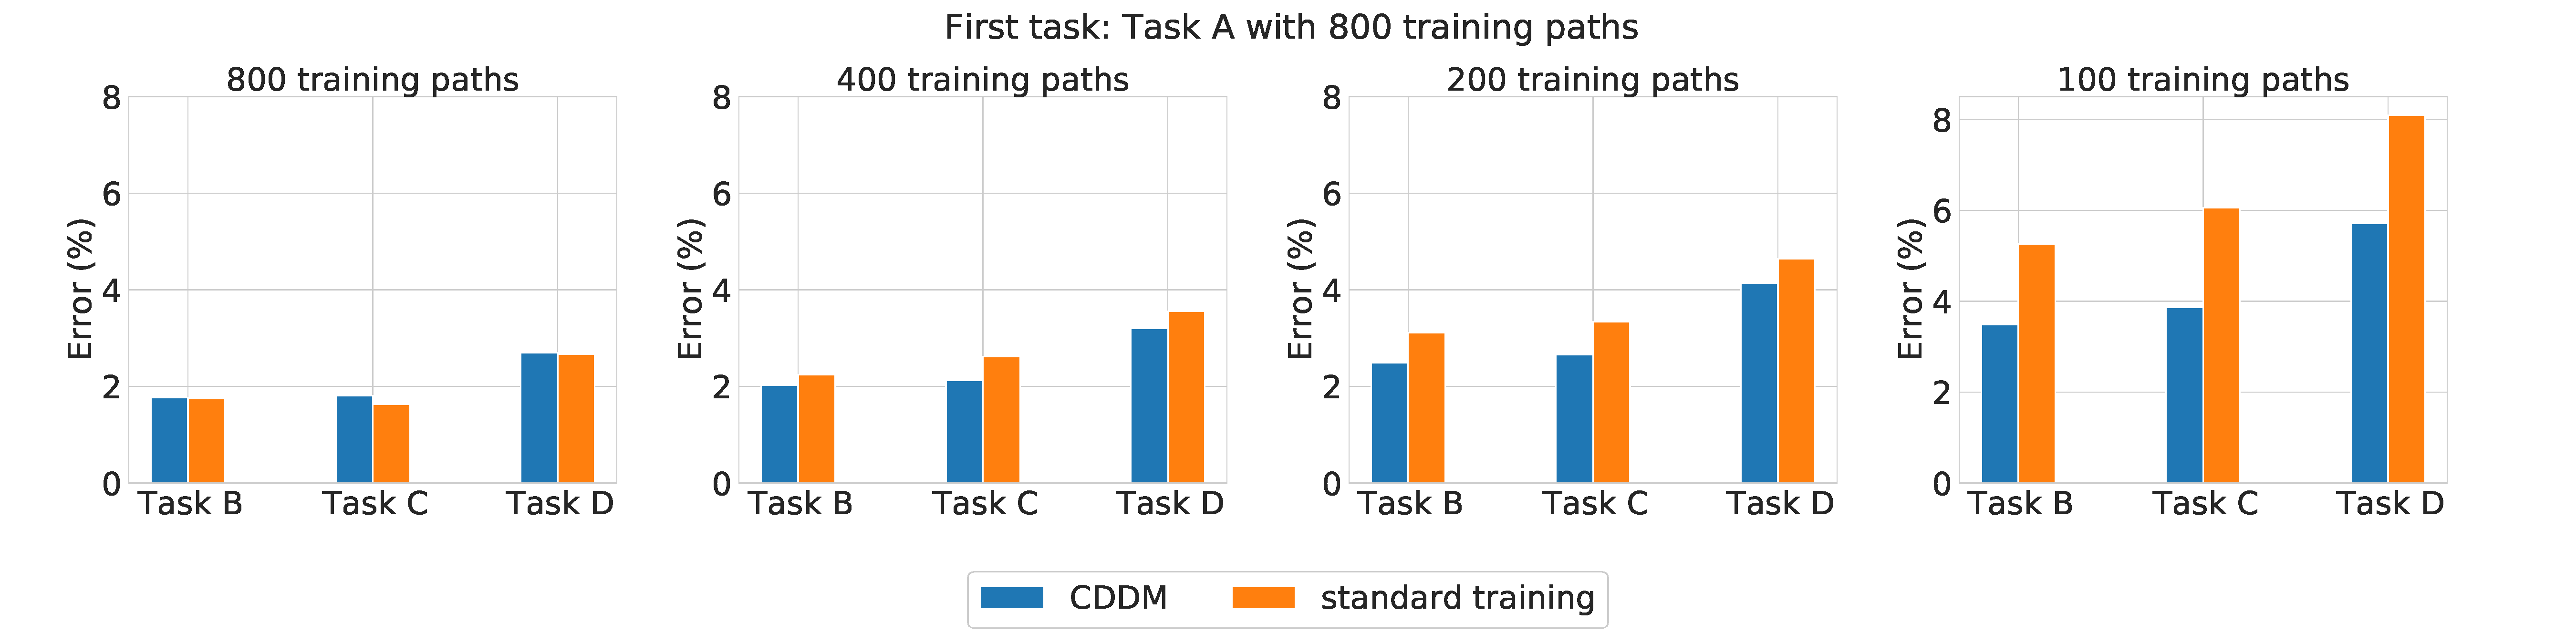
\includegraphics[width=\textwidth]{figures/std_cl.pdf}
    \color{Pink} Same holds for other orderings as well! 
\end{frame}

\begin{frame}{Parameters}
    \centering
    \includegraphics<1>[width=0.9\textwidth]{figures/total_param.pdf}
    \includegraphics<2>[width=0.7\textwidth]{figures/overlap.pdf}
\end{frame}

\begin{frame}
	\centering
	\conc
\end{frame}

\section{Conclusion}
\begin{frame}{Conclusion}
  \centering
  \begin{itemize}
    \item Less number of parameters compared to standard learning.
    \item Ordering does not matter.
    \item Mostly better than standard learning especially in scarce data regime!
  \end{itemize}
\end{frame}

\begin{frame}{However}
  \centering
  \begin{itemize}
    \item Deep stuff is not for me!
    \item What happens for a much wider task variance?
    \item This strategy is limited by number of parameters.
  \end{itemize}
\end{frame}

\begin{frame}
	\centering
  \thnx
\end{frame}

\end{document}
